\documentclass[twoside,10pt,parskip=half,ngerman]{scrreprt}

%***********************************************************************
% include some libs
%***********************************************************************
\usepackage[utf8]{inputenc}
\usepackage{listings}
\usepackage{color}
\usepackage{fancyhdr}
\usepackage{rotating}
%\usepackage{titlesec}
\usepackage{mathptmx}
% \usepackage{helvet}
% \usepackage[scaled]{uarial} %TODO: check
\renewcommand*\familydefault{\sfdefault} %% Only if the base font of the document is to be sans serif
\usepackage[T1]{fontenc}
\usepackage{ngerman}
\usepackage{textcomp}
\usepackage[squaren]{SIunits}
\usepackage{graphicx}
\usepackage{url}
\usepackage{geometry}
\usepackage[absolute]{textpos}
\usepackage{amsmath}
\usepackage{makeidx}
\usepackage{colortbl}
\usepackage{pdflscape}
\usepackage{pdfpages}
\usepackage{tabularx}
\usepackage{lmodern}
\usepackage{longtable}
\usepackage{array}
\usepackage{float}
\usepackage{scrhack}
\usepackage[plainpages=false]{hyperref}
\usepackage{wallpaper} %\ThisTileWallPaper{}
\usepackage[square]{natbib} %für BibTeX Literaturverzeichnis


% We need lowercase cursive font
\usepackage{amsmath}
\usepackage{fontspec}
\usepackage{unicode-math}
\setmainfont{TeX Gyre Pagella}

% Any of the following work, and probably many more
\setmathfont{TeX Gyre Pagella Math}
%\setmathfont{TeX Gyre Termes Math}
%\setmathfont{STIX}
%\setmathfont{Asana Math}

\DeclareRobustCommand{\bbone}{\text{\usefont{U}{bbold}{m}{n}1}}

\DeclareMathOperator{\EX}{\mathbb{E}}% expected value




%***********************************************************************
% various styles
%***********************************************************************	

%create index
\makeindex

%define pagestyle
\pagestyle{fancy}

%use sans-serif font 
%\renewcommand{\familydefault}{\sfdefault}

%define page margin
\geometry{a4paper, top=30mm, left=30mm, right=30mm, bottom=30mm,headsep=10mm,footskip=10mm}

%textpos parameter
\setlength{\TPHorizModule}{30mm}
\setlength{\TPVertModule}{\TPHorizModule}
\textblockorigin{10mm}{10mm} % start everything near the top-left corner
\setlength{\parindent}{0pt}

%horizontal lines for titlepage 
\newcommand{\HRule}{\rule{\linewidth}{0.5mm}}

%reference to source items inlc source number
\newcommand{\srcref}[1]{\nameref{src:#1} \cite{#1}}

%header / footer 
\renewcommand{\headrulewidth}{0.3pt}
\renewcommand{\footrulewidth}{0.3pt}

\fancyhead[LO,RE]{} %clear headings for contents 
\fancyhead[RO,LE]{\nouppercase{\rightmark}} %right odd pages and left even pages
\fancyhead[LO,RE]{\MakeUppercase{\leftmark}} %left odd pages and right even pages
\fancyfoot[LE,RO]{\thepage} %page numbering
\fancyfoot[C]{} %clear centered page numbering 

%define some colors
\definecolor{gray}{rgb}{0.95,0.95,0.95}
\definecolor{darkgray}{rgb}{0.4,0.4,0.4}
%listing colors
\definecolor{lgray}{RGB}{250,250,250}
\definecolor{lgreen}{RGB}{63,127,95}
\definecolor{lred}{RGB}{127,0,85}
\definecolor{lblue}{RGB}{42,0,255}

%***********************************************************************
% listing
%***********************************************************************

\lstset{		
		basicstyle=\small\ttfamily,
		frame=single,
		numbers=left,	
		numberstyle=\tiny,
		%firstnumber=auto,
		numberblanklines=true,
		captionpos=b,
		extendedchars=true,
		float=ht,
		showtabs=false,
		tabsize=2,
		showspaces=false,
		showstringspaces=false,
		breaklines=true,
		%prebreak=\Righttorque,
		backgroundcolor=\color{lgray},
		keywordstyle=\color{lred}\bfseries, 
		commentstyle=\color{lgreen}\ttfamily,
%		morekeywords={printstr, printhexln},
		stringstyle=\color{lblue},
		xleftmargin=0.5cm,
		xrightmargin=0.5cm
}

\lstloadlanguages{C++}

%\lstdefinelanguage{xc}{
%     keywords={printstr, printhexln, attributes, class, classend, do, empty, endif, endwhile, fail, function, functionend, if, implements, in, inherit, inout, not, of, operations, out, return, set, then, types, while, use},
%     keywordstyle=\color{lred}\bfseries,
%     ndkeywords={},
%     ndkeywordstyle=\color{yellow}\bfseries,
%     identifierstyle=\color{black},
%     sensitive=false,
%     comment=[l]{//},
%     commentstyle=\color{lgreen}\ttfamily,
%     string=[l]{"},
%     stringstyle=\color{lblue}\ttfamily
%  }



\begin{document}
\bibliographystyle{ieeetran}

\title{Projektarbeit 2019}
\author{Dano Roost & Ralph Meier}


\begin{titlepage}

% Logo
\ThisTileWallPaper{\paperwidth}{\paperheight}{images/logos/InIT.pdf} % {images/logos/*.pdf}
% Wählen Sie aus folenden pdf Files: ICP, IDP, IEFE, IMES, IMPE, IMS, INE, InES, InIT, KSR, SoE, ZAMP, ZAV, ZIL, ZPP, ZSN

\begin{minipage}[b]{0.117\textwidth}
\hskip 0.05cm
\end{minipage}
\begin{minipage}[b]{0.91\textwidth}
\begin{tiny}.\end{tiny}\vskip 2.8cm
	{\huge
	
	% Projekt Name
	\textbf{\underline{Project thesis (Computer Science)}}\\

	% Projekt Titel
	Reinforcement Learning mit einem Multi-Agenten System für die Planung von Zügen
	\vskip 0.5cm}
	
	\begin{minipage}[b]{0.27\textwidth}
	\hrule\vskip 0.5cm
		\textbf{Authors}\\
		\\
	\end{minipage}
	\begin{minipage}[b]{0.03\textwidth}
	\hskip 0.5cm
	\end{minipage}
	\begin{minipage}[b]{0.7\textwidth}
	\hrule\vskip 0.5cm
		Dano Roost\\
		Ralph Meier\\
	\end{minipage}
	
	\begin{minipage}[b]{0.27\textwidth}
	\hrule\vskip 0.5cm
		\textbf{Main supervisor}\\
		\\
	\end{minipage}
	\begin{minipage}[b]{0.03\textwidth}
	\hskip 0.5cm
	\end{minipage}
	\begin{minipage}[b]{0.7\textwidth}
	\hrule\vskip 0.5cm
		Andreas Weiler\\
        \\
	\end{minipage}
	
	\begin{minipage}[b]{0.27\textwidth}
	\hrule\vskip 0.5cm
		\textbf{Sub supervisor}\\
		\\
	\end{minipage}
	\begin{minipage}[b]{0.03\textwidth}
	\hskip 0.5cm
	\end{minipage}
	\begin{minipage}[b]{0.7\textwidth}
	\hrule\vskip 0.5cm
		Thilo Stadelmann\\
    \\
	\end{minipage}
	
	\begin{minipage}[b]{0.27\textwidth}
	\hrule\vskip 0.5cm
		\textbf{Date}
	\end{minipage}
	\begin{minipage}[b]{0.03\textwidth}
	\hskip 0.5cm
	\end{minipage}
	\begin{minipage}[b]{0.7\textwidth}
	\hrule\vskip 0.5cm
		20.12.2019
	\end{minipage}
\end{minipage}
\vskip 0.5cm
\end{titlepage}

\setcounter{page}{1}
%%%%%%%%%%%%%%%%%%%%%%%%%%%%%%%%%%%%%%%%%%%%%%%%%%%%%%%%%%%%%%%%%%
%  _____   ____  _____                                          %
% |_   _| /  __||  __ \    Institute of Computitional Physics   %
%   | |  |  /   | |__) |   Zuercher Hochschule Winterthur       %
%   | |  | (    |  ___/    (University of Applied Sciences)     %
%  _| |_ |  \__ | |        8401 Winterthur, Switzerland         %
% |_____| \____||_|                                             %
%%%%%%%%%%%%%%%%%%%%%%%%%%%%%%%%%%%%%%%%%%%%%%%%%%%%%%%%%%%%%%%%%
%
% Project     : LaTeX doc Vorlage für Windows ProTeXt mit TexMakerX
% Title       : 
% File        : Kontakt.tex Rev. 00
% Date        : 23.4.12
% Author      : Remo Ritzmann
% Feedback bitte an Email: remo.ritzmann@pfunzle.ch
%
%%%%%%%%%%%%%%%%%%%%%%%%%%%%%%%%%%%%%%%%%%%%%%%%%%%%%%%%%%%%%%%%%

\textbf{Kontakte}


\textbf{Vorlagen Ersteller} \\
M.Sc. Engineering ZHAW Remo Ritzmann \\
Wissenschaftliche Assistent Optoelectronic Research Laboratory\\
School of Engineering\\
Technikumstrasse 9, TL419\\
CH-8408 Winterthur

Phone: +41 (0)52 534 48 62\\
Zentrale: +41 (0)58 934 73 06\\
Mobile: +41 (0)79 830 17 35\\
E-Mail: remo.ritzmann@zhaw.ch\\
E-Mail Privat: remo.ritzmann@pfunzle.ch\\
Homepage: \url{http://www.icp.zhaw.ch}\vskip 15pt

%%%%%%%%%%%%%%%%%%%%%%%%%%%%%%%%%%%%%%%%%%%%%%%%%%%%%%%%%%%%%%%%%
%  _____   ____  _____                                          %
% |_   _| /  __||  __ \    Institute of Computitional Physics   %
%   | |  |  /   | |__) |   Zuercher Hochschule Winterthur       %
%   | |  | (    |  ___/    (University of Applied Sciences)     %
%  _| |_ |  \__ | |        8401 Winterthur, Switzerland         %
% |_____| \____||_|                                             %
%%%%%%%%%%%%%%%%%%%%%%%%%%%%%%%%%%%%%%%%%%%%%%%%%%%%%%%%%%%%%%%%%
%
% Project     : LaTeX doc Vorlage für Windows ProTeXt mit TexMakerX
% Title       : 
% File        : abstract.tex Rev. 00
% Date        : 23.4.12
% Author      : Remo Ritzmann
% Feedback bitte an Email: remo.ritzmann@pfunzle.ch
%
%%%%%%%%%%%%%%%%%%%%%%%%%%%%%%%%%%%%%%%%%%%%%%%%%%%%%%%%%%%%%%%%%

\thispagestyle{empty}
\chapter*{Zusammenfassung}\label{chap.zusammenfassung}

%1. Einleitung («Problemstellung»): Definiert die Problematik und begründet die Relevanz der Arbeit. Die Situation (eine problematische Situation oder technische Problematik) und die wissenschaftliche/fachliche Untersuchungs-Fragestellung (folgt logischer- weise aus der festgestellten Problematik) werden kurz beschrieben.
Die steigende Anzahl der Pendler bring die Kapazität des Schienennetzes der Schweizerischen Bundesbahnen SBB immer mehr an seine Grenzen. Da der Ausbau der Infrastruktur nicht mit den Passagierzahlen mithalten kann, bemüht sich die SBB, mehr Züge in dichteren Abständen auf ihr Netz zu bringen.
Für die Planung des dichteren Zugverkehrs experimentiert die SBB auch mit Technologien des maschinellen Lernens, insbesondere mit Reinforcement Learning (RL). Dabei soll ein Algorithmus selbstständig Strategien erlernen, um das gegebene Problem zu lösen. In diesem Fall handelt es sich dabei um das Steuern von Zügen, welche möglichst zeitnah zu ihrem Ziel geführt werden sollen. Kollisionen gilt es dabei zu verhindern und potenzielle Hindernisse wie defekte Züge müssen umfahren werden. Auch können Züge mit verschiedenen Geschwindigkeiten unterwegs sein, was bei der Planung berücksichtigt werden soll.\\
Diese Arbeit ist dabei ein Beitrag zur sogenannten Flatland Challenge, einem Wettbewerb der SBB und der Crowdsourcing-Plattform AICrowd, bei welchem das beschriebene Problem mittels einer zur Verfügung gestellten Simulation des Schienennetzes gelöst werden soll. Der Wettbewerb ist aufgeteilt in zwei Runden mit wachsendem Schwierigkeitslevel.
Diese Schienensimulation erlaubt es, eigene Lösungen für das Problem zu trainieren und zu evaluieren. Die Schwierigkeit dabei ist, die Züge so zu steuern, dass sie sich auch in komplexen Situationen nicht blockieren. Dazu ist primär die Zusammenarbeit der Züge von grosser Bedeutung.\\
%3. Vorgehen («Problembehandlung»): Informiert über das Vorgehen und über die Untersuchungsanlage.
Der präsentierte Lösungsansatz verwendet den Asynchronous Advantage Actor Critic Algorithmus (A3C), einer der derzeit besten RL-Algorithmen, welcher verteiltes Lernen ermöglicht. Der präsentierte Ansatz orientiert sich dabei stark an der Ausgangslösung von Stephan Huschauer.
Nach der ersten lauffähigen Version wurde der Ansatz nach und nach mit unterschiedlichen Features erweitert, wie beispielsweise einem veränderten Kontrollmechanismus der Züge, Curriculum Learning oder verteiltem Lernen über mehrere Rechner.
Um den Fortschritt zu quantifizieren wurden für sämtliche Änderungen Experimente durchgeführt. Durch das Hinzufügen unterschiedlicher Features konnte eine signifikante Verbesserung der Performanz verzeichnet werden. In Runde 1 war es dabei möglich, die Ankunftsrate von den 16.6\% der Ausgangslösung auf 48.9\% zu verbessern.
Für die anspruchsvolleren Eisenbahnnetze der 2. Runde, für welche keine Ausgangslösung existiert, konnte dank weiteren Verbesserungen ebenfalls ein respektables Resultat erzielt werden. Die präsentierte Lösung konnte eine Ankunftsrate von 29.1\% erreichen, was zum Evaluierungszeitpunkt dem 4. Platz von insgesamt 24 teilnehmenden Teams entsprach. Für einen praktischen Einsatz ist die präsentierte Lösung jedoch noch nicht geeignet, dies bedarf weiterer Forschung.
\NewPage
\thispagestyle{empty}
\chapter*{Abstract}\label{abstract}
The increasing number of commuters is pushing the capacity of the Swiss Federal Railways (SBB) rail network to its limits. Since the expansion of the infrastructure cannot keep up with the increasing number of passengers, SBB is exploring new ways to bring more trains onto its network. To achieve this goal, SBB is also experimenting with machine learning technologies such as reinforcement learning (RL). 
The goal for this type of algorithm is to independently learn strategies  in order to solve the problem at hand, in our case the challenge of guiding trains to their assigned destinations. Besides not colliding with other trains, it is also necessary to avoid potential obstacles such as defective trains and to take different speed profiles into account.\\
This work is a contribution the Flatland Challenge, a competition published by SBB and the crowdsourcing platform AICrowd, which aims to solve the problem described by using a provided simulation of the rail network. The competition is divided into two rounds with increasing difficulty. This rail simulation allows to train and evaluate own solutions for the given problem. The main task is to control the trains in cooperative way so they do not block each other even in complex situations. The selected solution uses the Asynchronous Advantage Actor Critic Algorithm (A3C), a state of the art RL algorithm which supports distributed learning. The approach presented is based on the baseline solution presented by Stephan Huschauer. After establishing the first running version, the approach was improved with an array of new features such as a modified train control mechanism, curriculum learning or distributed learning over multiple computers. To quantify the progress, experiments were conducted for all applied changes. By adding these features, a significant improvement could be achieved. In round one it was possible to improve the train arrival rate from 16.6\% of the baseline solution to 48.9\%.
For the more demanding second round, there is no baseline available. The solution presented was able to achieve a train arrival rate of 29.1\%, which corresponded at submission time to the 4th place of a total of 24 participating teams.
However, the solution presented is not yet suitable for practical use and requires further reseach to achieve a useful performance in a real world scenario.

\chapter*{Preface}\label{preface}
We would like to give special thanks to:
\begin{itemize}
    \item Andreas Weiler and Thilo Stadelmann for their great support during this work, for their helpful tips and for pushing us into the right direction.\\
    We are grateful for the opportunity to dive deep into the field of reinforcement learning as part of this project.
    \item Remo Maurer for being very generous with providing computing infrastructure, especially the infrastructure test server.
\end{itemize}



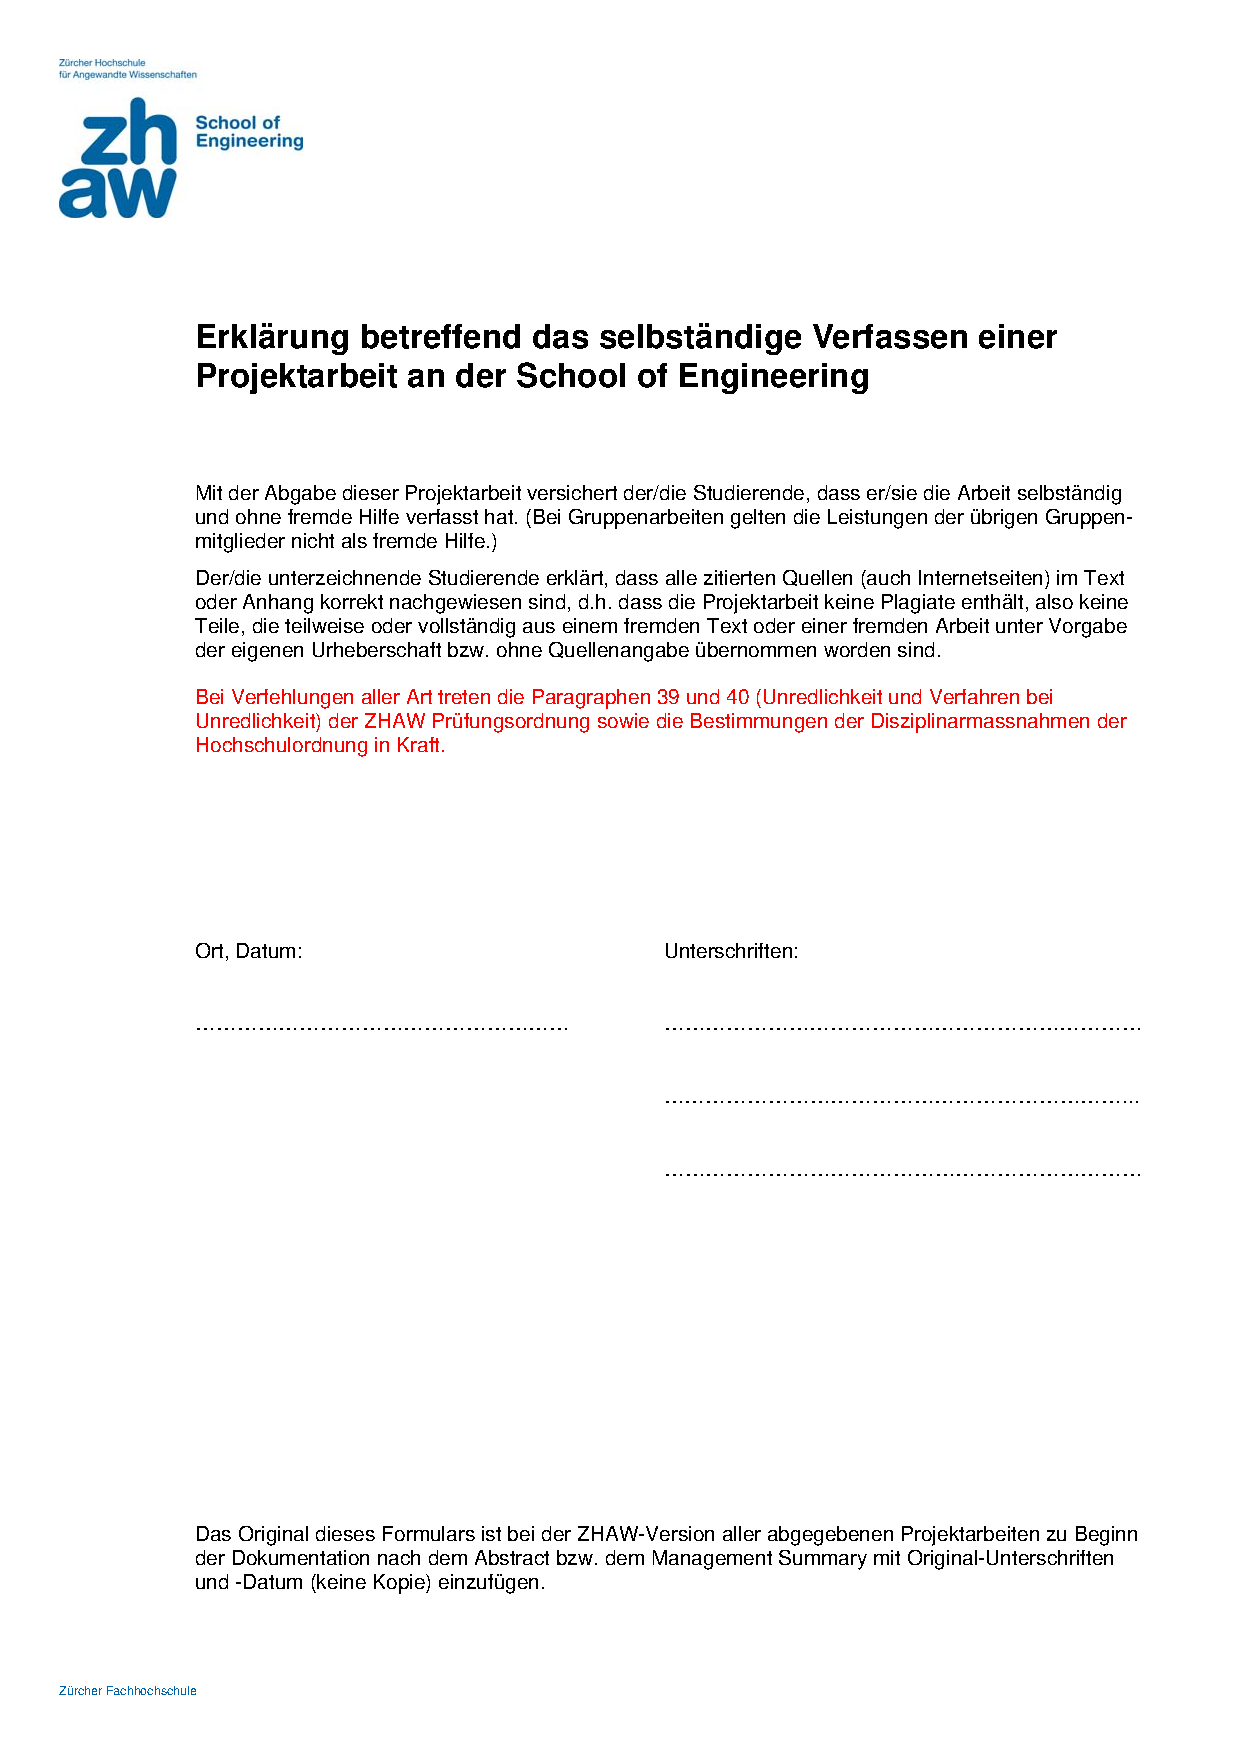
\includepdf{images/Erklaerung_PA.pdf} % Entsprechendes auskommentieren
% 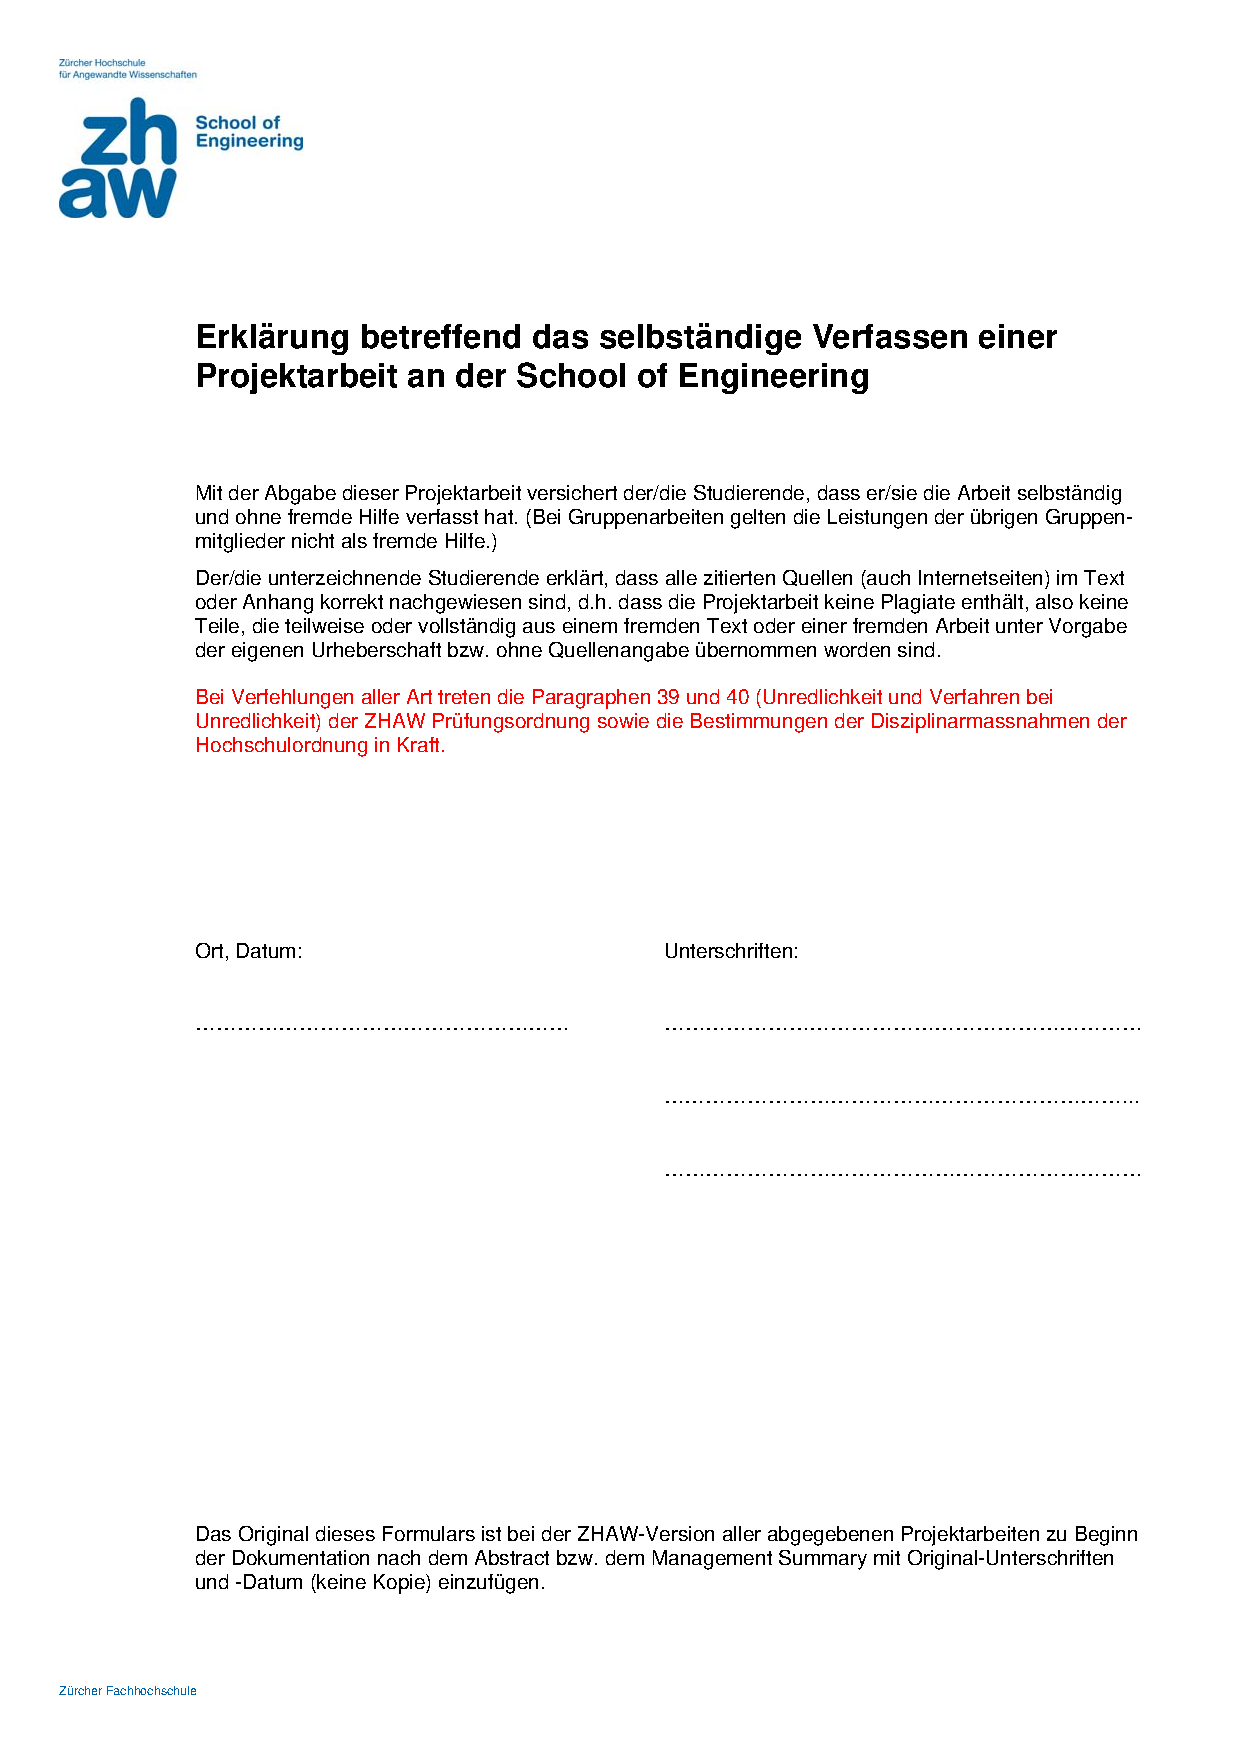
\includepdf{images/Erklaerung_PA.pdf}
% \newpage

%Inhaltsverzeichnis
\tableofcontents
\newpage



%\textbf{}
%\setcounter{page}{1}
%\pagenumbering{arabic}

%%%%%%%%%%%%%%%%%%%%%%%%%%%%%%%%%%%%%%%%%%%%%%%%%%%%%%%%%%%%%%%%%%
%  _____   ____  _____                                          %
% |_   _| /  __||  __ \    Institute of Computitional Physics   %
%   | |  |  /   | |__) |   Zuercher Hochschule Winterthur       %
%   | |  | (    |  ___/    (University of Applied Sciences)     %
%  _| |_ |  \__ | |        8401 Winterthur, Switzerland         %
% |_____| \____||_|                                             %
%%%%%%%%%%%%%%%%%%%%%%%%%%%%%%%%%%%%%%%%%%%%%%%%%%%%%%%%%%%%%%%%%
%
% Project     : LaTeX doc Vorlage für Windows ProTeXt mit TexMakerX
% Title       : 
% File        : header.tex Rev. 01
% Date        : 05.06.2012
% Author      : Remo Ritzmann
% Feedback bitte an Email: remo.ritzmann@pfunzle.ch
%
%%%%%%%%%%%%%%%%%%%%%%%%%%%%%%%%%%%%%%%%%%%%%%%%%%%%%%%%%%%%%%%%%

\chapter{LaTeX Kurzanleitung}\label{chap.anleitung}
Dieses Kapitel führt mit Beispielcode in den LaTeX Code ein, und kann während der Erstellung des Dokuments gelöscht werden.\footnote{Verbesserungsvorschläge bitte an remo.ritzmann@pfunzle.ch senden}

Die nachfolgende Berichtstruktur wurde aus der Vorlage\footnote{Berichtstruktur Vorlage, Stand: August 2011} der \href{https://intra.zhaw.ch/departemente/school-of-engineering/studium-standort-winterthur/studierende/projektarbeit-bachelorarbeit.html}{PA/BA Termin-Webseite} vom ZHAW Intranet entnommen.

(): alle in Klammer aufgeführten Einträge sind situativ anzupassen



Das ist ein kleiner Text um zu zeigen, wie die Enter eingebracht werden.\\
Ich finde Latex schwierig.\\
Der Start ist echt eine Herausforderung. \\
Mensch ist das Komplex, echt was für Profis. % Hier brauchts ja kein Enter mehr, sonnst heisst es Overfull \hbox



\section{Visio Vektorgraphik einfügen}\label{visio}
(Graphik auswählen) Speichern unter -> PDF -> Optionen.. -> Auswahl\\
Mit Adobe Akrobat öffnen: Erweitert -> Druckproduktion -> Seiten beschneiden -> Weisse Ränder entfernen -> OK -> Ctrl-S

\begin{figure}[H]
	\centering
		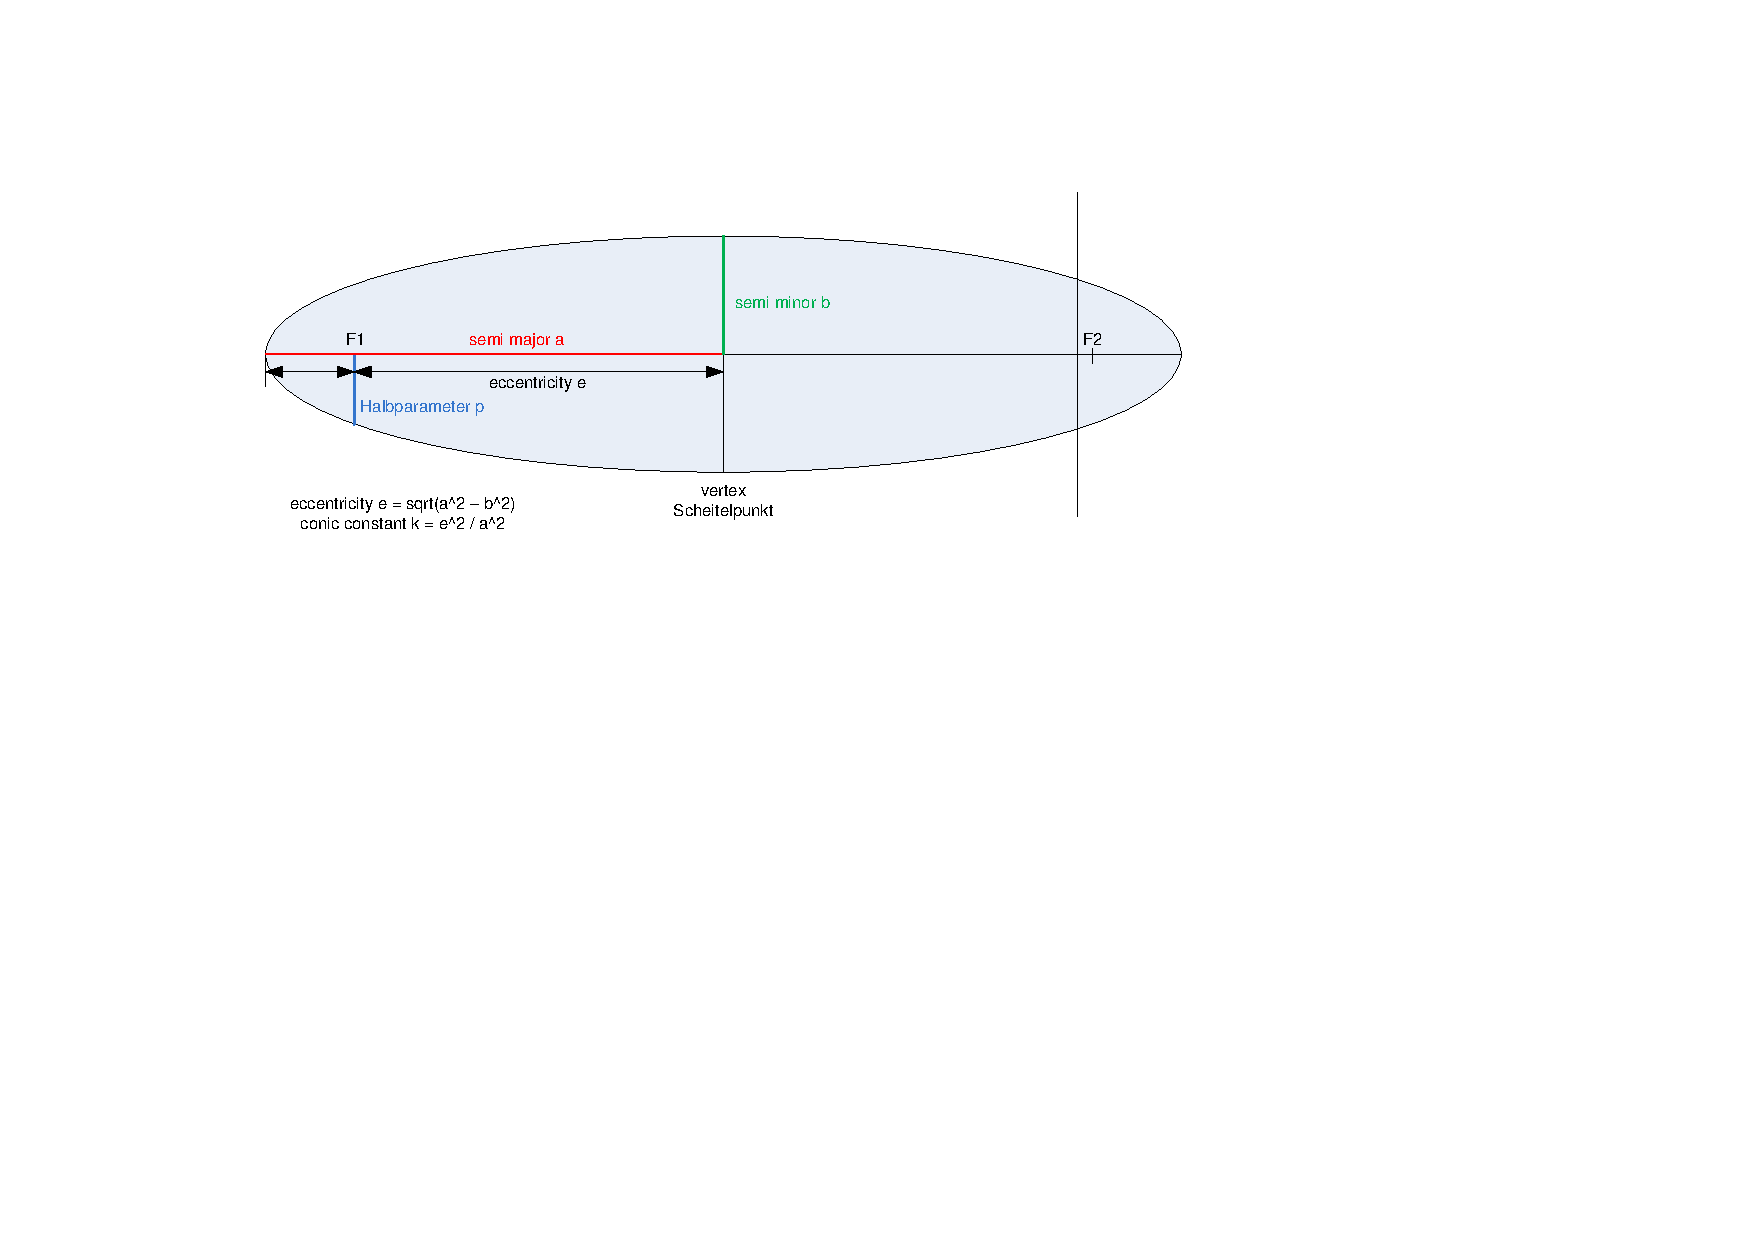
\includegraphics[width=0.8\textwidth]{images/visio/visio.pdf}
	\caption{Ideenskizze}
	\label{fig.Skizze}
\end{figure}

So kann die Abbildung~\ref{fig.Skizze} referenziert werden. Bei der PDF Erstellung ist darauf zu achten, dass LaTeX nur Versionen bis 1.4 voll unterstützt. 



\subsection{Graphiken in LaTeX zuschneiden}\label{zuschneiden}
Mit dem Befehl Clip kann eine Graphik auch in LaTeX zugeschnitten werden:

\begin{figure}[H]
	\centering
		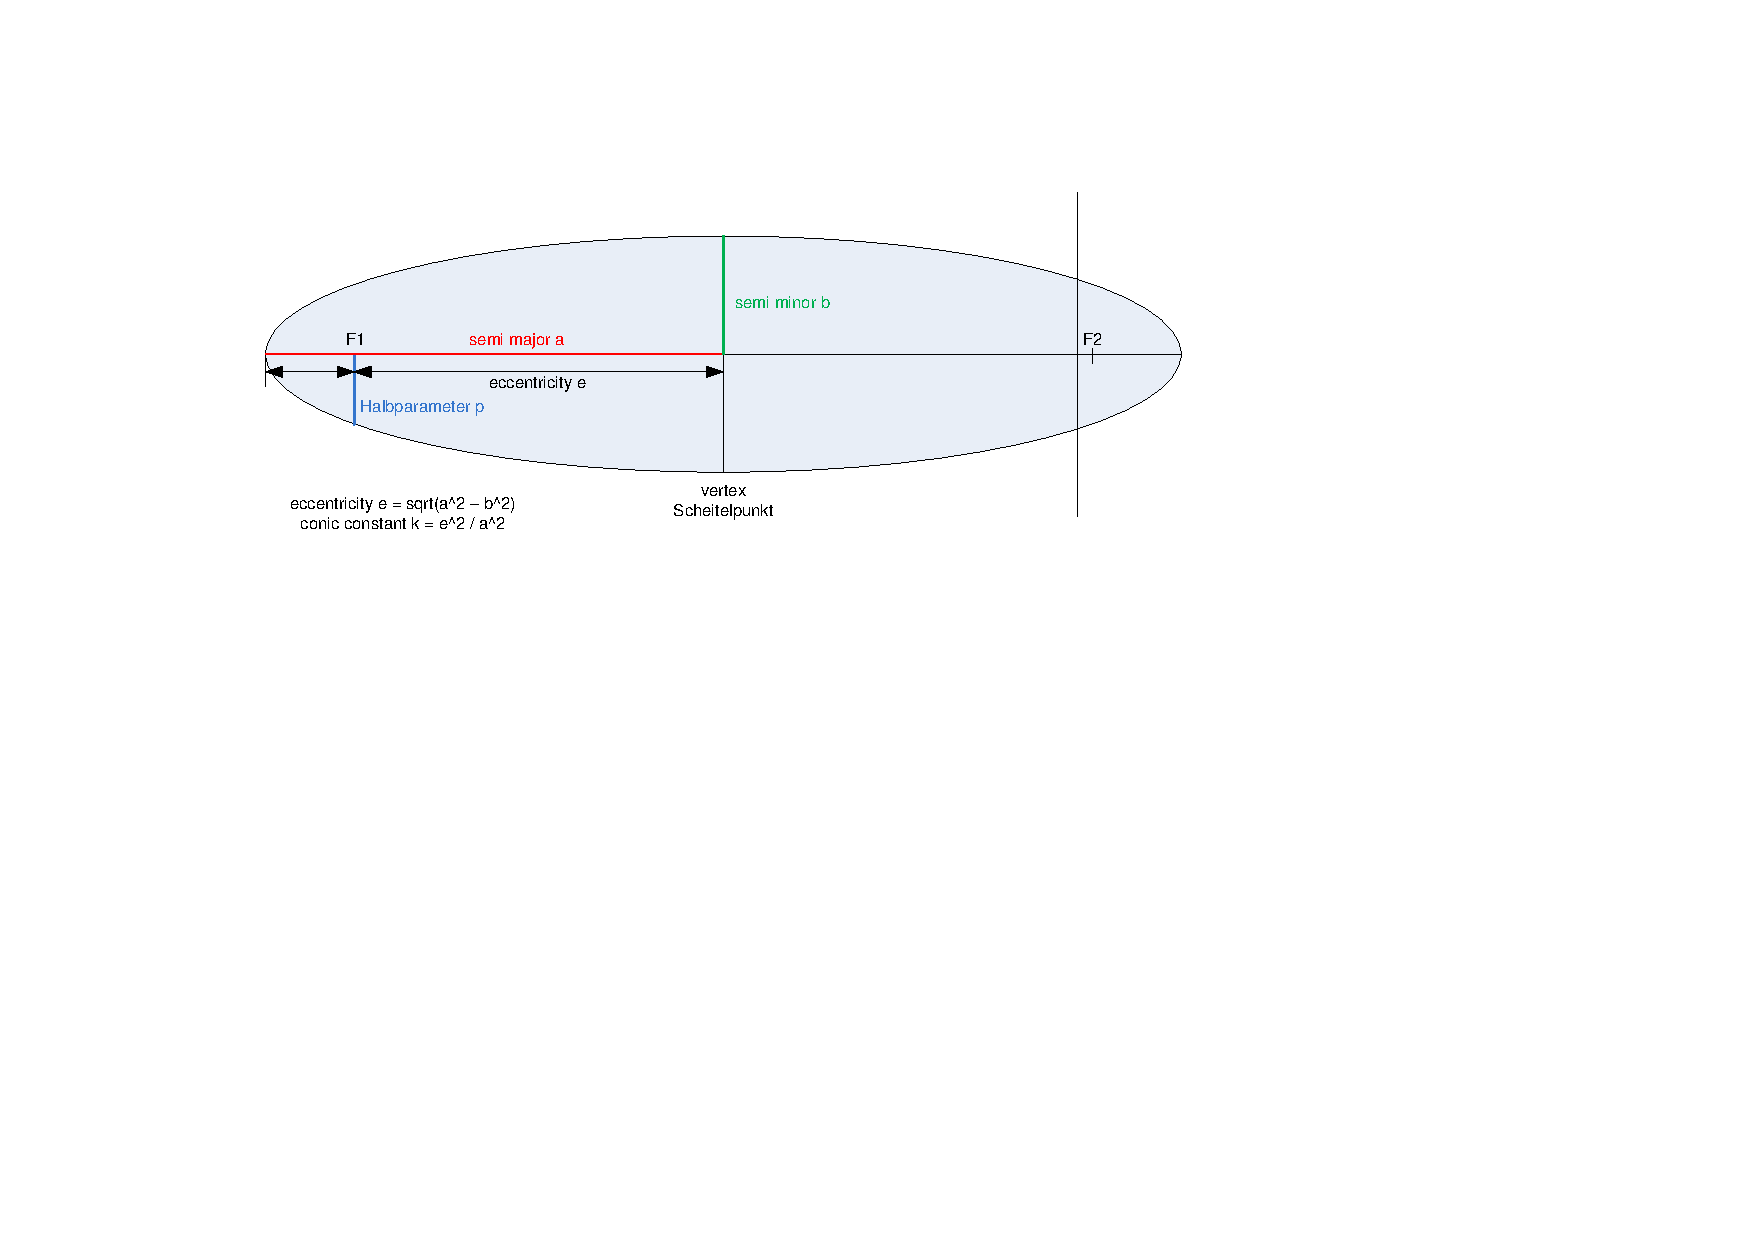
\includegraphics[width=0.9\textwidth, clip=true, trim = 80 10 0 10]{images/visio/visio.pdf}  % trim lm bm rm tm (left, bottom, right, top)
	\caption{clip=true, trim = 60 10 0 10}
	\label{fig.SkizzeZugeschnitten}
\end{figure}



\subsection{Mehrere Bilder nebeneinander}\label{nebeneinander}
Dank Minipages können mehrere Bilder auch nebeneinander sein:

%Zwei Bilder nebeneinander http://latex.mschroeder.net/
\begin{figure}[H]
  \centering
  \begin{minipage}[b]{0.45\textwidth}
    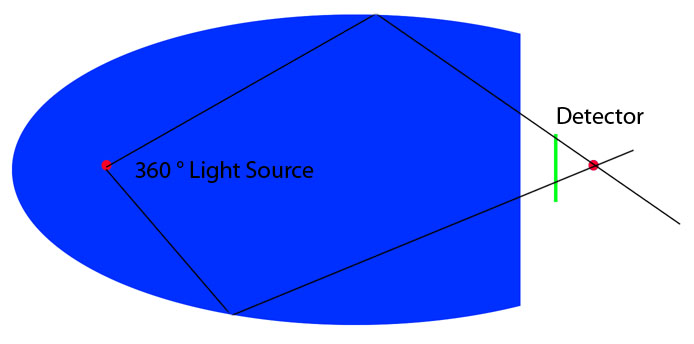
\includegraphics[scale=0.15]{images/photoshop/Skizze.jpg}
    \caption{Visir10b Detector}
    \label{Visir10bDetector} 
  \end{minipage} % Hier darf keine Leerzeile zwischen den beiden Minipages liegen!
  \begin{minipage}[b]{0.45\textwidth}
    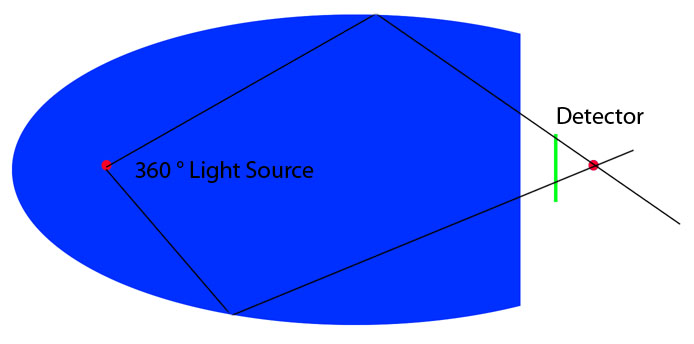
\includegraphics[scale=0.15]{images/photoshop/Skizze.jpg} 
    \caption{Visir10b Model}
    \label{Visir10bModel} 
  \end{minipage}
  \caption{Visir 10 mit optimiertem Reflektor}
  \label{fig.Visir10b}
\end{figure}


Literaturverweis: \citep[S.21]{analog_devices_dac}

\section{Tabellen aufbauen}\label{tabelle}
Kleine Tabelle:

\begin{table}[ht] \centering
	\begin{tabular}{|p{3cm}|p{.5cm}|p{.5cm}|p{.5cm}|p{.5cm}|p{.5cm}|p{.5cm}|p{.5cm}|p{.5cm}|p{.5cm}|p{.5cm}|} \hline
		\rowcolor{gray} Modul & M01 & M02 & M03 & M04 & M05 & M06 & M07 & M08 & M09 & M10 \\
		\hline
		FPGA\_DATEN & & & & & X & X & & X & X & \\
		\hline
		IRQ & X & X & X & & X & & & & X & X \\
		\hline
		Nachbar Core & & & & X & & X & & X & & \\
		\hline
	\end{tabular}
	\caption{Port Schwierigkeiten der Funkmodule}
	\label{tab:portprobleme}
 \end{table}	

Die nachfolgende longtable kann sich über mehrere Seiten erstrecken.

\begin{longtable}{|p{1.1cm}|p{4cm}|p{4cm}|p{4cm}|} 
					\hline
					\rowcolor{gray} Typ & Variante A & Variante B & Variante C
					\\ \hline
					& \textbf{Vorteile:} 
							\begin{itemize}
								\item[+] hohe Spannungen
							\end{itemize}							
							\textbf{Nachteile:}
							\begin{itemize}
								\item[-] Grosse Abmessung
							\end{itemize}
					& 	\textbf{Vorteile:} 
							\begin{itemize}
								\item[+] einfache Montage
							\end{itemize}							
							\textbf{Nachteile:}
							\begin{itemize}
								\item[-] max. 2A Eingangsstrom
							\end{itemize}
					&	\textbf{Vorteile:} 
							\begin{itemize}
								\item[+] hoher Strom
							\end{itemize}							
							\textbf{Nachteile:}
							\begin{itemize}
								\item[-] max. 12 V Eingangsspannung
							\end{itemize}\\ \hline
						Zeit & 2 h & 5 h & 3 h \\ \hline
						Preis	& 520 CHF/Stück & 800 CHF/Stück &	360 CHF/Stück\\ \hline
				\caption{Morphologischer Kasten für die Speisung}
				\label{tab:morphkasten}
			\end{longtable}	

Diese Art von Tabelle erstreckt sich immer auf der ganzen Seitenlänge:

\begin{tabularx}{\textwidth}{XXl}
  Salat & Schnecke & Igel\\
  Montag & Hier ist ein langes Wort & Dienstag
\end{tabularx}



\section{Code Listings aufbauen}\label{listing}

\begin{lstlisting}[
    language=C++,
    caption={Test Kommandozeilen Ausgabe},
    label={list.Testoutput}
]
/********************************************************/
/* Name        : M07Setup                               */
/* Description : EM9201 init for adress and pck         */
/* Input       : targetadr (DevAdr_M00 - DevAdr_M39)    */
/*               drate (Drate_M00 - Drate_M39)          */
/* Ouput       : -0x01 -> Setup OK                      */
/*               -0x5E -> Setup Error Channel write     */
/*               -0x6E -> Setup Error power write       */
/*               -0x7E -> Error in Device Address       */
/*               -0x8E -> Error in Peer Address         */
/********************************************************/
\end{lstlisting}

Formula $e = \sqrt{a{^2} - b^{2}}$


Diese Textstelle ist sehr interessant.\label{interessant}\\
Hier wird auf die Textstelle~\ref{interessant} verwiesen, die sich auf der Seite~\pageref{interessant} befindet.


% nogo:
% \ref{src:miktex} (\nameref{src:miktex})



\section{Citation nach IEEE}\label{citation}

Das ist ein \cite{robotvision} Verweis aufs Literaturverzeichnis. Ein anderes Beispiel ist das hier \cite{randompatterns}.





Das ist eine Aufzählung:
\begin{itemize} %
	\item Erste Zeile
	\item Zweite Zeile
	\item Dritte Zeile
\end{itemize}


\begin{enumerate}
\item erstens
\item zweitens
\end{enumerate}

%https://parma.zhaw.ch/svn/zhw_latex/
%gmanstyle nötig unter start od begin einbinden


Das ist eine verschachtelte Aufzählung:
\begin{description}
		\item [Register Performance] Alle Signale die das FPGA nicht verlassen, also von FF zu FF weitergeleitet werden. Daraus ergibt sich die maximale Taktfrequenz F\textsubscript{MAX}.

		\item [Externes Timing] FPGA Ein- und Ausgänge
		\begin{itemize}
			\item Ausgänge = Von FF's durch Logik zu Ausgängen (t\textsubscript{CO})
			\item Eingänge = Von Eingängen durch Logik zu FF's (t\textsubscript{SU}, t\textsubscript{H})
			\item Durchgänge = kombinatorische Pfade durch das FPGA (t\textsubscript{PD})
		\end{itemize}
\end{description}
 % Für das Schlussdokument auskommentieren

\chapter{Introduction}\label{chap.einleitung}
\section{Baseline}\label{baseline}
This work explores a real world usage of multi agent reinforcement learning (MARL) for controlling train traffic in a complex railway system.
As part of the Flatland challenge, a contest created by the Swiss Federal Railways (SBB) and the crowdsourcing platform AICrowd \cite{aicrowd}, we try to improve the performance of RL based train guidance and rescheduling. The goal of the challenge is to successfully guide all trains to their assigned target stations in a simulated environment called Flatland environment.
This is challenging because a single wrong decision can cause a chain reaction that makes it impossible for many other trains to successfully reach their destinations. The endeavor is further complicated by trains with different speed profiles and the possibility of malfunctioning trains. In the words of SBB and AICrowd, the challenge is described as follows \cite{aicrowd}:
\begin{quote}
	The Flatland Challenge is a competition to foster progress in multi-agent reinforcement learning for any re-scheduling problem (RSP). The challenge addresses a real-world problem faced by many transportation and logistics companies around the world (such as the Swiss Federal Railways, SBB). Different tasks related to RSP on a simplified 2D multi-agent railway simulation must be solved. Your contribution may shape the way modern traffic management systems (TMS) are implemented not only in railway but also in other areas of transportation and logistics. This will be the first of a series of challenges related to re-scheduling and complex transportation systems.
\end{quote}
The challenge consists of two parts \cite{aicrowd}.  
\begin{itemize}
	\item Part 1 includes avoiding conflicts with multiple trains (agents) on a given environment. The difficulty thereby is, that the layout of the environment is not known upfront.
	\item Part 2 aims to optimize train traffic which includes trains with different speed profiles, malfunctioning trains, less switchover facilities and in general more scheduled trains in a shorter time.
\end{itemize}
This work is based on the work of Stephan Huschauer \cite{flatlandstephan} and further investigates on the idea to use the asynchronous advantage actor critic algorithm (A3C) \cite{a3c}, a state of the art RL algorithm, to solve the task.
Besides the work of S. Huschauer, this work is also related to the work of Bacchiani, Molinari and Patander \cite{marltraffica3c}. Their work also aims to apply the A3C algorithm in a cooperative multi-agent environment and investigates communication free cooperation.
Unlike the Flatland challenge, the goal of this work is to cooperate on a road traffic environment. By applying the A3C algorithm, the work shows that it is possible learn cooperation by treating the other agents as part of the environment. Both the works of Bacchiani, Molinari and Patander as well as the work of S. Huschauer use a shared policy for all acting agents.

\section{Goal of this work}\label{zielsetzung}
%Comment: Explore ths use of A3C RL Learning in am cooperative multi agent env.
The aim of the work is to explore the use of the A3C algorithm in the Flatland multi-agent environment and to improve on the approach of S. Huschauer \cite{flatlandstephan}.\\
While there are better ways to solve the given problem than reinforcement learning, we mainly focus on pure RL but give our intution in \autoref{chap.resultate} on how the explored approach could work together with other techniques to improve its success.
This work is targeted towards an audience with a brief understanding of deep reinforcement learning. A basic introduction into the topic is given in \autoref{reinforcementlearning}. This introduction is focused on the techniques required to understand the applied A3C algorithm and does not cover the whole field of RL.
Also, the details of the Flatland environment can be found in \autoref{flatland_intro}. For a deeper understanding of the complex Flatland environment, it is recommended to study the Flatland documentation and specification \cite{flatland_docu} as well as the official Flatland introduction \cite{aicrowd}.

\section{Iterative Work Approach}\label{basic_cons}
We divide this work into 4 main sections:
\begin{itemize}
	\item \textbf{\nameref{chap.basic_implementation}:} We have a look at our basic implementation to solve the Flatland challenge. Also, we shortly describe the technologies used.
	\item \textbf{\nameref{chap.experiment}:} We identify parts of the implementation that offer room for improvement. To verify our work, we create experiments and analyse them afterwards.
	\item \textbf{\nameref{chap.resultate}:} We discuss out final solution that we submit in the Flatland challenge for both round 1 and round 2.
	\item \textbf{\nameref{chap.diskussion}:} We analyse parts of our solution that would need further improvement.
\end{itemize}
We take the idea of using the A3C algorithm to solve the Flatland problem and try various modifications in an attempt to improve its performance. We proceed by giving an idea, what we want to achieve, followed by an experiment setup and an experiment analysis to either prove or disprove our hypothesis. We do this in an iterative manner, to gradually come closer to a well-performing solution for Flatland.\\
In our experiments, we focus exclusively on Flatland round 2. While we compare our solution for round 1 with the baseline from S. Huschauer in \autoref{chap.resultate}, all technical improvements have also become part of our solution for round 2.

%%%%%%%%%%%%%%%%%%%%%%%%%%%%%%%%%%%%%%%%%%%%%%%%%%%%%%%%%%%%%%%%%
%  _____   ____  _____                                          %
% |_   _| /  __||  __ \    Institute of Computitional Physics   %
%   | |  |  /   | |__) |   Zuercher Hochschule Winterthur       %
%   | |  | (    |  ___/    (University of Applied Sciences)     %
%  _| |_ |  \__ | |        8401 Winterthur, Switzerland         %
% |_____| \____||_|                                             %
%%%%%%%%%%%%%%%%%%%%%%%%%%%%%%%%%%%%%%%%%%%%%%%%%%%%%%%%%%%%%%%%%
%
% Project     : LaTeX doc Vorlage für Windows ProTeXt mit TexMakerX
% Title       : 
% File        : grundlagen.tex Rev. 00
% Date        : 7.5.12
% Author      : Remo Ritzmann
% Feedback bitte an Email: remo.ritzmann@pfunzle.ch
%
%%%%%%%%%%%%%%%%%%%%%%%%%%%%%%%%%%%%%%%%%%%%%%%%%%%%%%%%%%%%%%%%%

\chapter{Technical and Theoretical Foundation}
\label{chap.grundlagen}
\chaptermark{Foundations}
\section{Reinforcement Learning}\label{reinforcementlearning}
\subsection*{Basic Definitions}\label{basic_rl_definitions}
In recent years, major progress has been achieved in the field of reinforcement learning (RL) \cite{mnih2013playing,alphazero,hideandseek}.
In RL, an agent learns to perform a task by interacting with an environment $\mathcal{E}$. On every timestep $\mathcal{t}$ the agent $\mathcal{a}$ needs to take an action $\mathcal{u}$. The selection of this action $\mathcal{u}$ is based on the current observation $\mathcal{s}$. The success of the agent is measured by reward $\mathcal{R}$ received. If the agent does well, it receives positive reward from the environment, if it does something bad, there is no or negative reward.
\begin{figure}[H]
	\centering
	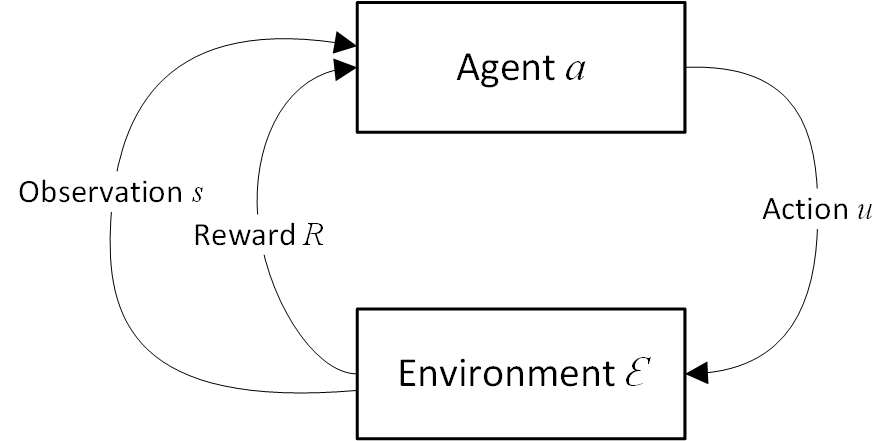
\includegraphics[width=250pt]{images/rl_overview.png}
	\caption{Reinforcement learning overview}
\end{figure}
The goal of the agent is now to take an action that maximizes the expected reward for all future timesteps $\EX[\mathcal{R}_{t+1}+\mathcal{R}_{t+1}+\mathcal{R}_{t+1}+...|\mathcal{s}_{t}]$ given the current observation $\mathcal{s}$.\\
This estimation should be as close as possible to the sum of actually received rewards. Often, these received rewards are discounted with a constant factor $\mathcal{\gamma}$ to the power of timestep $\mathcal{t}$. With $\mathcal{\gamma}$ being something slightly less than 1, this accounts for the fact that rewards far in the future are hard to estimate.
The current observation $\mathcal{s}_{t}$, also known as the current state is used to determine which action $\mathcal{u}$ to take next. An agent can observe its environment either fully or partially. The cycle of taking actions and receiving a new state is repeated until the environment has reached a terminal state. Each rollout of such an environment is called an episode.
\subsection*{Value Based vs. Policy Gradient Based Methods}\label{value_policy_based_methods}
Reinforcement learning methods are categorized into value-based methods and policy gradient-based methods \cite{tdlearning},\cite{policygradient}. Those variants differ on how they select an action $\mathcal{u}$ from a given state $\mathcal{s}$.\\
Value-based RL algorithms work by learning a value function $\mathcal{V(s)}$ through repeated rollouts of the environment. $\mathcal{V(s)}$ aims to estimate the future expected reward for any given state $\mathcal{s}$ as precisely as possible. Using this approximation $\mathcal{V(s)}$ we can now select the action $\mathcal{u}$ that takes the agent into the next state $\mathcal{s}_{t+1}$ with the highest expected future reward. This estimation $\mathcal{V(s)}$ is achieved by either a lookup table for all possible states or a function approximator. In this work, we solely focus on the case that $\mathcal{V(s)}$ is implemented in form of a neural network as function approximator. To train the neural network, we try to minimize the squared difference between the estimated reward $\mathcal{V(s)}$ and the actual reward:
\begin{gather*}
loss_{value}=(\mathcal{R}-\mathcal{V(s)})^2
\end{gather*}
In some value-based algorithms such as Deep Q-Networks \cite{mnih2013playing}, a $\mathcal{Q(s,u)}$-function is used. This function tries to estimate the expected future reward on taking action $\mathcal{u}$ from the given state $\mathcal{s}$.\\
The second category of reinfocement learning algrithms are the so called policy gradient based methods. These methods aim to aquire a stochastic policy $\pi$ that maximizes the expected future reward $\mathcal{R}$ by taking actions with certain probabilities. Taking actions based on probabilities solves an important issue of value based methods, which is, that by taking greedy actions with respect to state  $\mathcal{s}$, the agent might not explore the whole state space and misses out on better ways to act in the environment.

\subsection*{Asynchronous Advantage Actor Critic Algorithm (A3C)}\label{a3c_intro}
The progress in RL has led to algorithms that combine value based and policy gradient based methods , generally known as actor-critic algorithms. The \textit{asynchronous advantage actor critic algorithm} (A3C), developed by Mnih et al. \cite{a3c} fits into this category. It uses both a policy $\pi$ and a value function $\mathcal{V(s)}$.
Both are usually seperate function approximators (neural networks in our case).
\begin{itemize}
	\item The \textbf{actor} can be seen as the policy $\pi$, that selects the action $\mathcal{u}$ based on a state $\mathcal{s}$.
	\item The \textbf{critic} is the value function $\mathcal{V(s)}$ that estimates, how much reward can be expected from a certain state on.
\end{itemize}
To enhance the process of learning policy $\pi$, the policy loss gets multiplied by the difference between actually received reward $\mathcal{R}$ and the estimated future reward $\mathcal{V(s)}$. This difference is called the advantage $\mathcal{A}$.
\begin{gather*}
\mathcal{A}=\mathcal{R}-\mathcal{V(s)}
\end{gather*}
This advantage is then used to update the policy.
\begin{gather*}
loss_{policy}=log \pi(s_{t})*\mathcal{A}
\end{gather*}
For actions where the received reward $\mathcal{R}$ exceeds the expected reward $\mathcal{V(s)}$ the policy update gets multiplied by a positive advantage. Therefore, the update of the neural network gets adjusted into a direction that favors the experienced actions based on the seen states.\\
What makes A3C different from other actor-critic algorithms is, that it can be used in a distributed way. Many workers work at the same time on a centralized model. How we take advantage of this features is discussed in \nameref{dist_architecture}.

\section{The Flatland Rail Environment}\label{flatland_intro}
The Flatland environment is a virtual simulation environment provided by the Swiss Federal Railway SBB and the crowdsourcing platform AICrowd.
The goal of this environment is to act as a simplified simulation of real train traffic.
\begin{figure}[H]
	\centering
	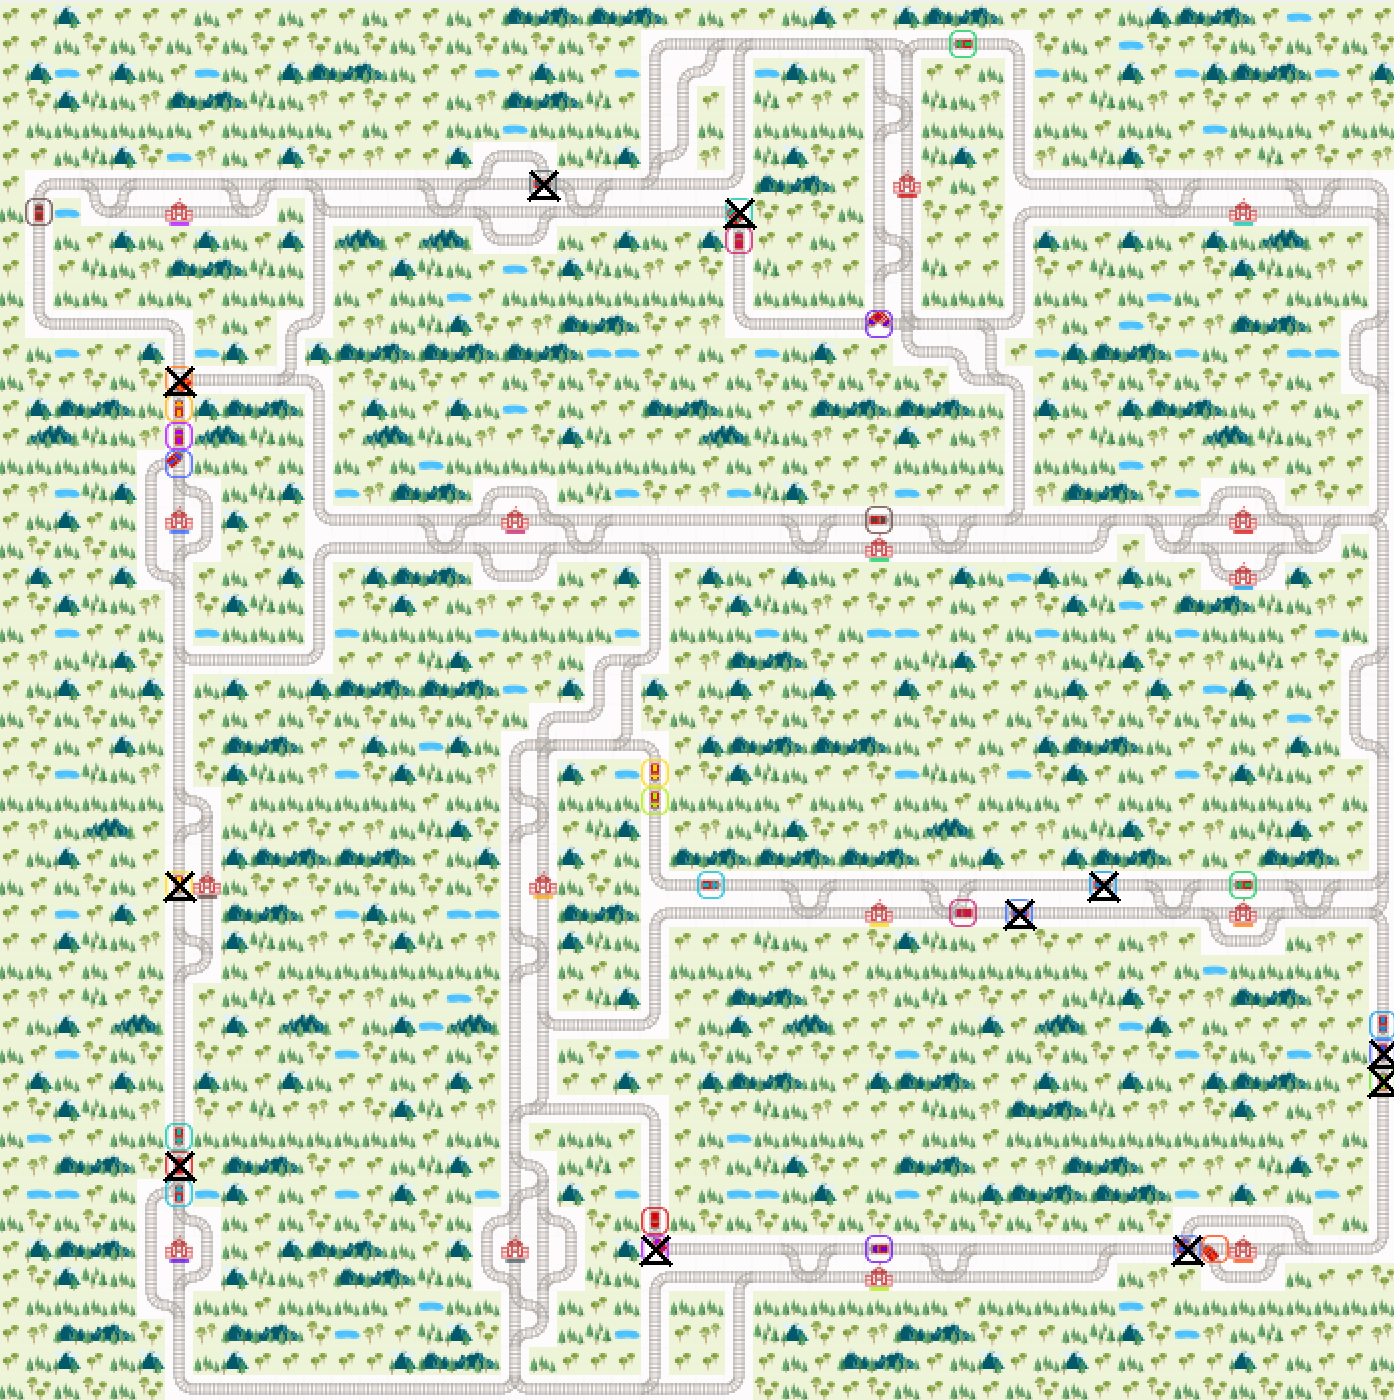
\includegraphics[width=300pt]{images/screenshot_flatland.png}
	\caption{Screenshot from a running Flatland environment.}
\end{figure}
Using Flatland, we can train RL algrithms to control the actions of trains, based on observations on the grid. Flatland has a discrete structure in both its positions and its timesteps. The whole rail grid is composed out of squares that can have connections to neighbouring squares. In certain squares, the rails splits into two rails. On those switches, the agent has to make a decision which action it wants to take. Dependent on the type of switch, there are different actions available.
\begin{figure}[H]
	\centering
	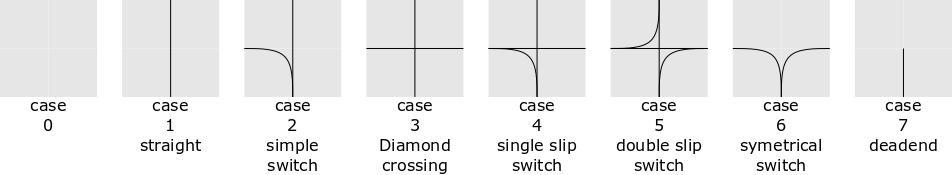
\includegraphics[width=300pt]{images/transition_nips_proposal.png}
	\caption{Possible switches in the Flatland environment from \cite{flatland_docu}.}
\end{figure}
An exception poses switches that are approached from a side that does not allow to take an action, e.g. approaching a \textit{case 2} switch from the north side.
All rail parts, independent of if it is a switch also allow to take the actions to do nothing (remain halted, or keep riding), to go forward or to brake.
The action space is therefore defined by:
\begin{gather*}
U = \{ \text{do nothing, go left, go forward, go right, brake} \}
\end{gather*}
It is important to note that trains do not have the ability to go backwards and therefore need to plan ahead to avoid getting stuck. To learn which actions to take, the agents have to learn to adapt to an unknown environment due to the fact that the environments are randomly generated and differ on each episode. Depending on the given parameters, the size and complexity of the grid can be adjusted. This allows for dynamically changing the difficulty for the agents.\\
The goal of each agent is to reach an assigned target train station as fast as possible. Agents that reach this destination are removed from the grid which means, they can no longer obstruct the path of other trains.

\subsection*{Observations}\label{observations}
The Flatland environment allows to create observation builders to observe the environment for each agent. While it is possible to observe the whole grid, this does usually not make sense due to the fact that many parts of the rail grid are not relevant to a single train. Flatland offers by default two different observation builders.\\\\
\textbf{GlobalObsForRailEnv} creates three arrays with the dimensions of the rectangular rail grid. The first array contains the transition information of the rail grid. For each cells, there are 16 bit values, 4 bit for each possible direction a train is facing.\\\\
\textbf{TreeObsForRailEnv} creates a graph with sections of the grid as nodes from the perspective of the train.
This means, only the switches which the train is actually able to take define a single node. As an example, a train on a \textit{case 0} switch heading from north to south is not able to make a decision on this switch and therefore, the TreeObservation does not put the sections before and after the switch into two different nodes but just into a single node.\\
The nodes of the tree observation offer a number of fields that allow to select specific features to create numeric input vectors for function approximator such as neural networks. The tree observation builder offers 14 distinct features for each rail section. This includes:
\begin{itemize}
	\item Distance until own target encountered: Cell distance to the own target railway station. Infinitiv if target railway station for agent is not in this section.
	\item Distance to other agent encountered: Cell distance to the next other agent on this section.
	\item Distance to next branch: The length of this section.
	\item Min. distance to target: The minimal cell distance to the target after this section is finished.
	\item Child nodes: The nodes the agent is able to take after this section ends. Each child node is associated with a direction (left, forward, right).
\end{itemize}
\subsection*{Agent Evaluation}\label{rl_agent_eval}
AICrowd and SBB provide a system for agent evaluation. This system evaluates the policy on a number of unknown environments and outputs the percentage of agents that reached their assigned destination as well as the received reward while doing so. The evaluation reward scheme is thereby as follows \cite{flatland_faq}:
\begin{gather*}
R_{t}= 
\begin{cases}
-1,				& \text{if } s_{t} \text{ is not terminal}\\
10,             & \text{otherwise}
\end{cases}
\end{gather*}
The difficulty of the evaluation level does differ between round 1 and round 2. While round 1 offered many connecting rails between the starting position and the assigned target of an agent, round 2 has more sparse connections and usually only provides 2 to 4 rails between cities. The concept of cities has been added in round 2. Those differences can be clearly seen in \autoref{fig:eval_comp} with the densly connected environment for round 1 versus the sparsly connected environment for round 2. 
\begin{figure}[H]
	\centering
	\begin{subfigure}{.5\textwidth}
		\centering
		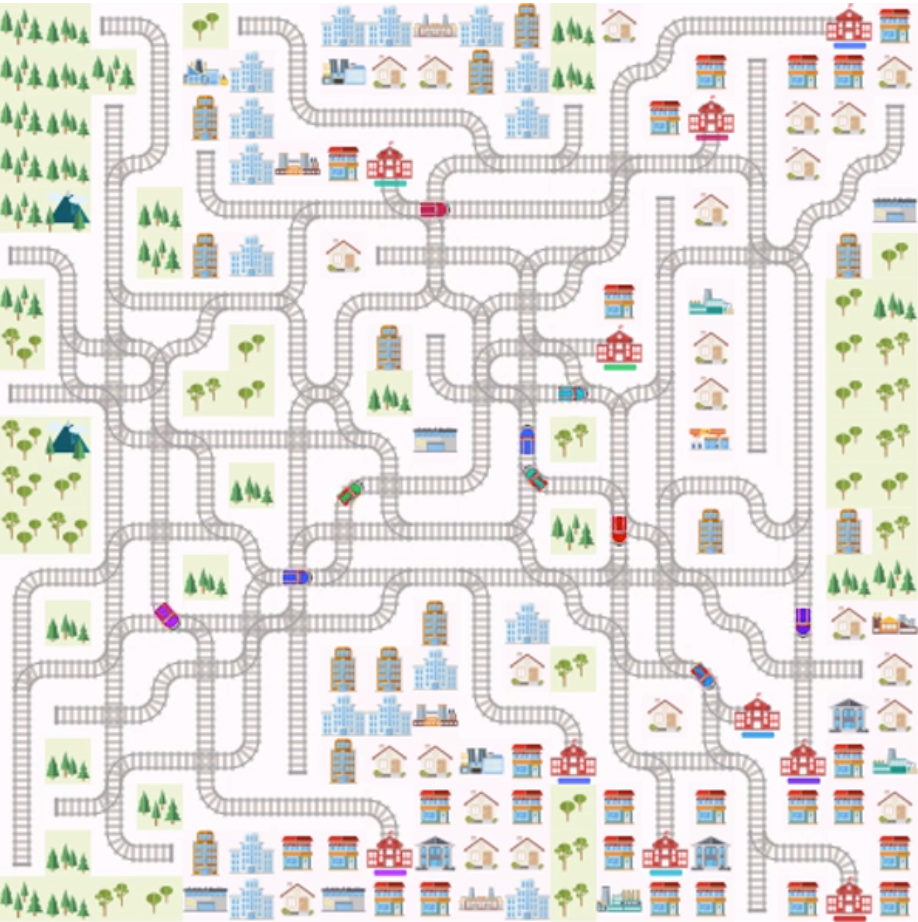
\includegraphics[width=200pt]{images/example_eval_round1.png}
		\caption{Evaluation round 1.}
		\label{fig:eval_round1}
	\end{subfigure}%
	\begin{subfigure}{.5\textwidth}
		\centering
		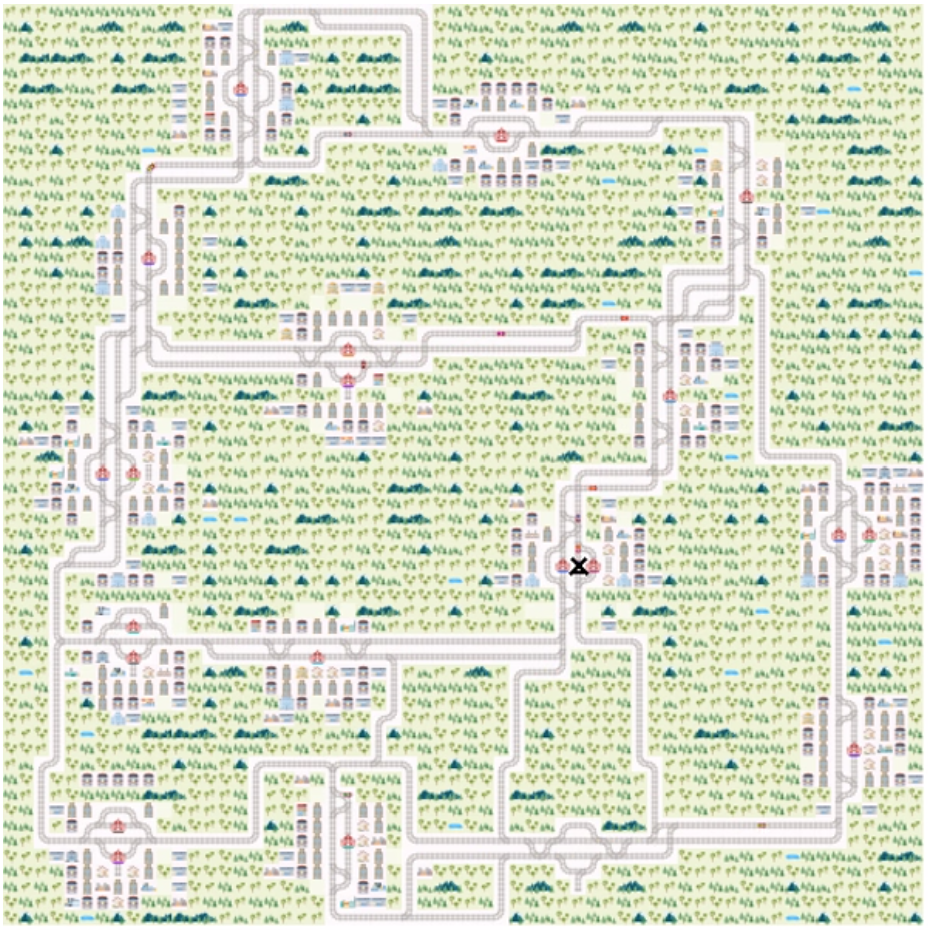
\includegraphics[width=200pt]{images/example_eval_round2.png}
		\caption{Evaluation round 2.}
		\label{fig:eval_round2}
	\end{subfigure}
	\caption{Comparison between two screenshots from evaluation environments from Flatland round 1 and round 2.}
	\label{fig:eval_comp}
\end{figure}



 % (2. Theoretische Grundlagen)
%%%%%%%%%%%%%%%%%%%%%%%%%%%%%%%%%%%%%%%%%%%%%%%%%%%%%%%%%%%%%%%%%
%  _____   ____  _____                                          %
% |_   _| /  __||  __ \    Institute of Computitional Physics   %
%   | |  |  /   | |__) |   Zuercher Hochschule Winterthur       %
%   | |  | (    |  ___/    (University of Applied Sciences)     %
%  _| |_ |  \__ | |        8401 Winterthur, Switzerland         %
% |_____| \____||_|                                             %
%%%%%%%%%%%%%%%%%%%%%%%%%%%%%%%%%%%%%%%%%%%%%%%%%%%%%%%%%%%%%%%%%
%
% Project     : LaTeX doc Vorlage für Windows ProTeXt mit TexMakerX
% Title       : 
% File        : vorgehen.tex Rev. 00
% Date        : 7.5.12
% Author      : Remo Ritzmann
% Feedback bitte an Email: remo.ritzmann@pfunzle.ch
%
%%%%%%%%%%%%%%%%%%%%%%%%%%%%%%%%%%%%%%%%%%%%%%%%%%%%%%%%%%%%%%%%%

\chapter{Approach and Methodology}\label{chap.vorgehen}
\section{Basic Considerations}\label{basic_cons}
As described under \autoref{baseline}, our work is based on the work of S. Huschauer \cite{flatland}. We take the idea of using the A3C algorithm to solve the flatland problem and try various modifications in an attempt to improve its performance.\\
We proceed by giving an intution, what we want to achieve by changing the specified part, followed by an experiment to either prove or disprove our hypothesis.\\
For training purposes, we started by reimplementing the algorithm by ourselfes. This enabled us from the beginning to gain a deeper understanding of how the algorithm works and where we could find possible areas for improvement. From there, we iteratively added these potential improvements to later compare them against the version without this feature.

\subsection*{Reproducability in Reinforcement Learning}\label{enhanced_observations}
It is important to note, that the training process of reinforcement learning and especially multi agent reinforcement learning is hard to evaluate and reproduce. Depending on the initial weights of the neural networks and the shape of the environments, the performance may vary on each restart. Also, the number of workers can 
significantly influence the training performance. To counter the latter, we execute all presented experiments on machines with the same specifications (see TODO-INFRASTRUCTURE).\\
Another point that is hard to reproduce is training stability. In A3C, an important instrument to prevent the policy from converging too early is using an additional entropy term. Our way to maintain stability with changing environments is discussed in \autoref{hy}.

\section{Reinforcement Learning for Flatland}
\subsection*{A3C Implementation}\label{enhanced_observations}
Originally, the asynchronous advantage actor critic algorithm (A3C) has been designed for use in a single agent environment \cite{a3c}.
By applying it in a multi agent environment, we implicitly convert the environment into a non-stationary environment.
While applying A3C in a multi agent setting, the other agents can be viewed as part of the environment. This means, the behaviour of the environment changes while training, due to the fact that the behaviour of the other agents changes.

Gupta et al. \cite{multiagent_comp_a3c_dqn_etc} finds, that RL methods like Deep-Q networks (DQN) and Trust region policy optimization (TRPO) are not performing well in a multi agent environment, due to the combination of experience replay and non-stationarity of the environment. We therefore suggest, that it is not recommendable to keep an experience replay buffer with older episodes. Otherwise the sampled experience might represent old agent behaviour which is then learned.

\subsection*{Observation Design}\label{enhanced_observations}
The flatland environment provides a base to build custom observation builders that can be used to create a state representation for the agents. Based on the provided TreeObsForRailEnv (see \autoref{observations}), we implement a custom observation builder which we use to produce an input vector to our neural network. This observation builder takes the the current state of the environment and produces a fixed size numeric vectors with values between 0 and 1 for each agent. This input vector should fulfil an number of requirements:
\begin{itemize}
	\item Each rail section the agent possibly rides on next should be visible to the agent.
	\item The agent should be able to detect, whether there is another train coming the opposite direction on any section.
	\item The agent should be able to detect on each switch which turn is closer to his target.
	\item On switches, the agent should be able to see if a turn does lead to his target, even if it is not the fastest way. If this is the case, taking this turn might even be a good option to evade possibly blocking situations.
	\item For the next grid tile, the agent should be able to detect if it is a switch and if so, if it is one the agent can make a decision on. (see \autoref{flatland_intro} for non-usable switches).
	\item 
\end{itemize}

\subsection*{Action Space Reduction and Script Policy Actions}\label{reduced_action_space}
The flatland environment is designed in a way to resemble a classical RL environment. This means, on every timestep, we receive observations for each agent, calculate an action and hand this action to the environment, visible in pseudocode \autoref{alg:no_reduction}. 


\begin{algorithm}[H]
	\KwData{initialized flatland environment $\mathcal{E}$, initial observation $\mathcal{s\SPSB{a}{t=0}}$ for all agents }
	\KwResult{terminal flatland environment}
	\While{episode not terminal}{
		create empty action array $\mathcal{A}$\\
		\For{every agent $\mathcal{a}$}{
			get current state $\mathcal{s\SPSB{a}{t}}$ of agent\\
			Fetch action  $\mathcal{u}$ for agent $\mathcal{a}$ at timestep $\mathcal{t}$ based on $\mathcal{s\SPSB{a}{t}}$ from policy $\pi$\\
			$\mathcal{A[a]}$ = $\mathcal{u}$
		}
		call $\mathcal{step(A)}$ of $\mathcal{E}$\\
		retrieve reward $\mathcal{R}$\\
		retrieve all new states $\mathcal{s_{t+1}}$\\
	}
	\caption{Default episode for flatland environment}
	\label{alg:no_reduction}
\end{algorithm}
While this makes sense in an environment where agents need to take an action on every timestep (such as Atari games), in flatland most of the time the only reasonable action is to move forward as visible in \autoref{fig:no_desicion}. Only around switches, the actions of an agent have acutual consequences.
\begin{figure}
	\centering
	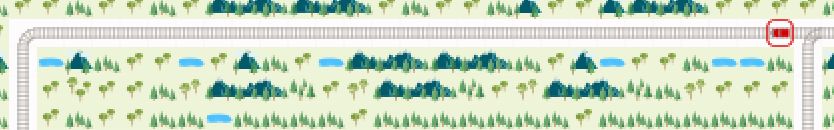
\includegraphics[width=300pt]{images/screenshot_no_decision.png}
	\caption{Screenshot from flatland environment. A train heading east. The only reasonable action is to ride forward.}
	\label{fig:no_desicion}
\end{figure}
Every action that is produced by the neural network should be included for training, so the network can adapt to this type of situation. The problem arises now, that all these actions of riding forward are included into the training of the agent. The influence of the actions that actually matter (e.g. the ones around switches) is thereby not as big as it could be, because a large portion of the training data is actually situations that do not actually require decisions.\\
To solve this problem, we implement hard coded rules that the agents follow as long as they are not in a situation to make a decision. Only around switches, the neural network policy is activated. As a consequence, the data used for training has less samples but the samples available are of higher quality. The training with this mechanism implemented looks like \autoref{alg:with_reduction}.
For training, we only use the experience collected near the switch.
\begin{algorithm}[H]
	\KwData{initialized flatland environment $\mathcal{E}$, initial observation $\mathcal{s\SPSB{a}{t=0}}$ for all agents}
	\KwResult{terminal flatland environment}
	\While{episode not terminal}{
		create empty action array $\mathcal{A}$\\
		\For{every agent $\mathcal{a}$}{
			\eIf{agent is near to a switch}{
				get current state $\mathcal{s\SPSB{a}{t}}$ of agent\\
				Fetch action  $\mathcal{u}$ for agent $\mathcal{a}$ at timestep $\mathcal{t}$ based on $\mathcal{s\SPSB{a}{t}}$ from policy $\pi$\\
				$\mathcal{A[a]}$ = $\mathcal{u}$
			}{
				$\mathcal{A[a]}$ = $\mathcal{u_{forward})}$
			}
		}
		call $\mathcal{step(A)}$ of $\mathcal{E}$\\
		retrieve reward $\mathcal{R}$\\
		retrieve all new states $\mathcal{s_{t+1}}$\\
	}
	\caption{Improved learning for flatland environment}
	\label{alg:with_reduction}
\end{algorithm}
This drastically improves training performance as visible in .

// TODO: Chart


\subsection*{Curriculum Learning and Reward assignment}\label{curriculum_learning}
The reward assignment in flatland can be freely configured. But as long as there is not some distance-to-target dependent reward function, the probability, that an agent with an uninformed policy finds its target is small. This is especially the case for large environments with many trains on it. For example, most evaluation environments of flatland round 2 have up to 200 individual agents and are up 100x100 tiles large (SOURCE!). The rollout of such an environment takes a lot more time than the rollout of a 20x20 environment with 5 trains. Also, the probability, that a train arrives in a small environment is larger and therefore, the experience is more valuable for training.
To improve training times, it makes therefore sense to start with a small environment and move to larget ones, once the agents mastered pathfinding and basic collision avoidance.

\subsection*{Entropy Balancing and Hyperparameter Tuning}\label{entropy_balancing_hyperparameter}
In RL, it is of great importance to find the right combination of exploration and explotation. During exploration, the agent explores as much of the state space as possible. This enables the agent to later exploit the found states which are beneficial. Without this exploration, there is a chance that the agent settles on suboptimal policies too quickly and ignores parts of the state space the agent has never seen.\\
The policy is characterized by a probability distribution of actions.


\subsection*{Agent Communication}\label{reduced_action_space}
Communication in multi agent RL is a topic of active research and considered very complex


\section{Distrubuted Architecture and Parallelism}\label{dist_architecture}
Für die vorliegende Arbeit wurden die unten aufgeführten Programme eingesetzt.








\begin{itemize}
\item (Beschreibt die Grundüberlegungen der realisierten Lösung (Konstruktion/Entwurf) und die Realisierung als Simulation, als Prototyp oder als Software-Komponente)
\item (Definiert Messgrössen, beschreibt Mess- oder Versuchsaufbau, beschreibt und dokumentiert Durchführung der Messungen/Versuche)
\item (Experimente)
\item (Lösungsweg)
\item (Modell)
\item (Tests und Validierung)
\item (Theoretische Herleitung der Lösung)
\end{itemize}

\section{(Used Software)}\label{software}
We used the following tools in our project.

\subsection*{Working Environment}\label{os}
\begin{itemize}
	\item Microsoft Windows 10
	\item Ubuntu 19.04
\end{itemize}

\subsection*{Visual Studio Code}\label{vsc}
\begin{itemize}
	\item Visual Studio Code 1.40
\end{itemize}

\subsection*{Documentation}\label{dokutools}
\begin{itemize}
	\item XeLateX with Visual Studio Code
	\item XeLateX with WebStorm
\end{itemize}


\subsection*{Programming language}\label{programminglanguages}
\begin{itemize}
	\item Python 3.6
\end{itemize}

\subsection*{Python modules}\label{modules}
\begin{itemize}
	\item Flatland-rl 1.3 - 2.1.10
	\item Tensorboard 2.0
	\item Keras x.x
	\item Cython x.x
	\item %TODO: finish this
\end{itemize}


\section{Basic considerations}
%split into round 1 / round 2

\subsection{Round 1}
%Observations
%Convolutional network + Global observations
%Early stopping
%Reward vergabe angepasst
We started with rebuilding the A3C algorithm from S. Huschauer to get a better knowledge how A3C works.\\
We made some experiments with different observations: TreeObservations and GlobalOberservations.
Because we made better and faster progress with GlobalObservatione we continued with those and combind them with a convolutional network.
Right after starting this project, we faced a problem regarding the reward distribution.\\


\subsection{Round 2}




\section{Measurands}
%Messgrössen: Evaluator, benchmark

\section{Experiments}
%

\section{Solution approach}
%Neue Actions


\section{Testing and submissions}

\section{Theoretical derivation of the solution}



 % Vorgehen / Methoden
%%%%%%%%%%%%%%%%%%%%%%%%%%%%%%%%%%%%%%%%%%%%%%%%%%%%%%%%%%%%%%%%%
%  _____   ____  _____                                          %
% |_   _| /  __||  __ \    Institute of Computitional Physics   %
%   | |  |  /   | |__) |   Zuercher Hochschule Winterthur       %
%   | |  | (    |  ___/    (University of Applied Sciences)     %
%  _| |_ |  \__ | |        8401 Winterthur, Switzerland         %
% |_____| \____||_|                                             %
%%%%%%%%%%%%%%%%%%%%%%%%%%%%%%%%%%%%%%%%%%%%%%%%%%%%%%%%%%%%%%%%%
%
% Project     : LaTeX doc Vorlage für Windows ProTeXt mit TexMakerX
% Title       : 
% File        : resultate.tex Rev. 00
% Date        : 23.4.12
% Author      : Remo Ritzmann
% Feedback bitte an Email: remo.ritzmann@pfunzle.ch
%
%%%%%%%%%%%%%%%%%%%%%%%%%%%%%%%%%%%%%%%%%%%%%%%%%%%%%%%%%%%%%%%%%

\chapter{Results}\label{chap.resultate}
\section{Round 1}
Our submission for Flatland round 1 does not include all algorithmic improvements discussed in this work. None the less, we were able to achieve a significant improvement in performance compared to the baseline version from \cite{flatlandstephan}.
Our submission for round 1 contains the following components:
\begin{itemize}
	\item Custom A3C implementation without experience replay buffer.
	\item Default TreeObsForRailEnv (in round 1, this was a numeric vector by default).
	\item Policy learned by curriculum learning.
	\item Distributed training over multiple processes on the same machine (no cross-machine distribution possible yet).
\end{itemize}
Using the performance evaluation system provided together with the Flatland environment, we reach the following performance metrics:


\begin{tabular}{ |c|c|c|c| } 
	\hline
	\textbf{Author} & \textbf{Observation type} & \textbf{Local Evaluation Score} & \textbf{Submission Score} \\
	\hline
	Stephan Huschauer & reduced grid observation & 19.4\% & 16.6\% \\
	& tree observation & 24.7\% & - \\
	We & tree observation & 69.3\% & 48.9\% \\
	\hline
\end{tabular}

%Vergleich mit Stefan:
%He used the first version of Flatland to evaluate his models and got a total score of 24.7\% in a local evaluation.
%He trained his model with 2 to 10 agents with a field of view of 10*10.

\section{Round 2}
Our submission for Flatland round 2 contains all in this work discussed improvements of the algorithm. While a direct comparison is difficult due to a lack of a baseline version for round 2, we could still show in our experiments how our adjustments to the implementation improved the performance of our algorithm.\\





%%%%%%%%%%%%%%%%%%%%%%%%%%%%%%%%%%%%%%%%%%%%%%%%%%%%%%%%%%%%%%%%%
%  _____   ____  _____                                          %
% |_   _| /  __||  __ \    Institute of Computitional Physics   %
%   | |  |  /   | |__) |   Zuercher Hochschule Winterthur       %
%   | |  | (    |  ___/    (University of Applied Sciences)     %
%  _| |_ |  \__ | |        8401 Winterthur, Switzerland         %
% |_____| \____||_|                                             %
%%%%%%%%%%%%%%%%%%%%%%%%%%%%%%%%%%%%%%%%%%%%%%%%%%%%%%%%%%%%%%%%%
%
% Project     : LaTeX doc Vorlage für Windows ProTeXt mit TexMakerX
% Title       : 
% File        : diskussion.tex Rev. 00
% Date        : 7.5.12
% Author      : Remo Ritzmann
% Feedback bitte an Email: remo.ritzmann@pfunzle.ch
%
%%%%%%%%%%%%%%%%%%%%%%%%%%%%%%%%%%%%%%%%%%%%%%%%%%%%%%%%%%%%%%%%%

\chapter{Discussion and Outlook}
\label{chap.diskussion}
\chaptermark{Discussion}
\section{Review of the Application of Reinforcement Learning}\label{discussion_rl}
While trying to solve the Flatland challenge with RL, we discovered a limitation of policy-gradient based methods in high-consequence environments like Flatland. 
We call Flatland a high-consequence environment because taking a bad action quickly leads to a chain reaction of unresolvable situations. Policy-based RL uses a possibility distribution over all available actions. This leads to the problem that even if the best action is taken with a possibility of 90\%, the remainig (probably non-beneficial actions) have a combined chance of 10\% to be selected. For 10 agents with such a possibility distribution, there is already a 65.1\% chance that one of the agents takes a non-beneficial action and creates a chain of problems. Just converting this probability distribution into a deterministic policy by using the $\mathcal{argmax}$ over the possibility distribution does not solve the problem due to some situations in which the agent is not sure what to do and therefore assigns similar possibilities to the actions. The algorithm then relies on its stochasticity to try all available actions. It would be therefore interresting to experiment with value-based RL algorithms to observe, if such algorithms can overcome the described problem that policy-methods have. In most popular use-cases of RL such as Atari games, it will suffice to just select a good action and not nescessarily the best. This is different in Flatland and should therefore be adressed.

\section{Practicability in a Real World Scenario}\label{discussion_real_world}
While we were able to greatly improve the performance of the presented solution compared to the given baseline, it is still nowhere near practical applicability. While the presented evaluation tasks probably do not represent the real world density on a rail network, also with a lower volume of traffic, train traffic would require more robust solutions with the primary objective of finding a solution for every train to reach its destination instead of optimizing the performance of a single agent.

\section{Ideas for Future Research}\label{discussion_research}
We think that in order to further improve performance, the problem would need to be formulated in a different way. While the research presented in this work was mainly focused on treating the trains as agents in a multi-agent reinforcement learning problem, it might be an interresting approach to instead introduce a centrally planning agent that takes over all planning in advance. Especially in an simulated environment like Flatland with perfect information, we think that upfront planning would have potential to take full advantage of the available data and the possibility to iterativly plan the upcoming steps. With all planning done by a single agent, it would also remove the requirement for communication. While we could show in \autoref{agent_communication} that it is possible to learn communication protocols between agents, we think that in a less constructed example the convergence towards a usable communication protocol might be too slow to actually use it in real-world training with many agents.\\
Combined with the possibilty of a centrally planning agent, we think that converting the rail network into a logical graph would enable any training algorithm to perform better without the need for respecting the tile-based architecture of the Flatland environment. In \autoref{reduced_action_space}, we already take a step in this direction by reducing the actions required for each agent. 

 % Diskussion und Ausblick

\chapter{Verzeichnisse}\label{chap.verzeichnisse}
% %%%%%%%%%%%%%%%%%%%%%%%%%%%%%%%%%%%%%%%%%%%%%%%%%%%%%%%%%%%%%%%%%
%  _____   ____  _____                                          %
% |_   _| /  __||  __ \    Institute of Computitional Physics   %
%   | |  |  /   | |__) |   Zuercher Hochschule Winterthur       %
%   | |  | (    |  ___/    (University of Applied Sciences)     %
%  _| |_ |  \__ | |        8401 Winterthur, Switzerland         %
% |_____| \____||_|                                             %
%%%%%%%%%%%%%%%%%%%%%%%%%%%%%%%%%%%%%%%%%%%%%%%%%%%%%%%%%%%%%%%%%
%
% Project     : LaTeX doc Vorlage für Windows ProTeXt mit TexMakerX
% Title       : 
% File        : literatur.tex Rev. 00
% Date        : 23.4.12
% Author      : Remo Ritzmann
% Feedback bitte an Email: remo.ritzmann@pfunzle.ch
%
%%%%%%%%%%%%%%%%%%%%%%%%%%%%%%%%%%%%%%%%%%%%%%%%%%%%%%%%%%%%%%%%%

Um ein automatisches Literaturverzeichnis mit der 
\href{http://www.zhaw.ch/de/zhaw/hochschulbibliothek/dienstleistungen/literaturverwaltung.html}{ZHAW Literaturverwaltung} oder \href{www.bit.ly/literaturverwaltung}{www.bit.ly/literaturverwaltung} zu erstellen, besuchen Sie die Seite \href{www.refworks.com/refworks}{www.refworks.com/refworks} und erstellen Sie ein neuer Account.

-> \textbf{Für ein neues Konto registrieren}

Bibliographi erstellen -> BibTeX auswählen

%In Einstellungen direkt zu BibTex
%http://scholar.google.ch/scholar_settings?hl=de&as_sdt=0,5



\begin{thebibliography}{99}
\addcontentsline{toc}{section}{Literaturverzeichnis}\label{cha:literaturverzeichnis}

% How to make a Literaturlist nach www.ieee.org/documents/ieeecitationref.pdf
% Erklärung







%Books
\bibitem{robotvision} B. Klaus and P. Horn, Robot Vision. Cambridge, MA: MIT Press, 1986.
%Einzelne Seiten aus Buch
\bibitem{randompatterns} L. Stein, ">Random patterns,"> in Computers and You, J. S. Brake, Ed. New York: Wiley, 1994, pp. 55-70.





%Reports

% Peridicals (Zeitschriften)



% Gibt es eine automatische Konvertierung von Bibtech to LaTeX?

% Alte Beispiele
\bibitem{miktex} Latex Programmiere Umgebung (basic-miktex-2.8.3582.exe)\\
\href{http://www.miktex.org/about}{miktex.org}, 28.03.2010

\bibitem{wireshark}Wireshark, Programm zur Darstellung von Ehternet Packeten\\
\href{http://www.wireshark.org/download.html}{http://www.wireshark.org/download.html}



\end{thebibliography}

\addcontentsline{toc}{section}{Literaturverzeichnis}\label{cha:literaturverzeichnis}
 \bibliography{BibTeX-Literaturverzeichnis/literatur}
 \listoffigures
 \addcontentsline{toc}{section}{(Abbildungsverzeichnis)}
 \listoftables
 \addcontentsline{toc}{section}{(Tabellenverzeichnis)}
% \addcontentsline{toc}{chapter}{(Symbolverzeichnis)}
 %%%%%%%%%%%%%%%%%%%%%%%%%%%%%%%%%%%%%%%%%%%%%%%%%%%%%%%%%%%%%%%%%
%  _____   ____  _____                                          %
% |_   _| /  __||  __ \    Institute of Computitional Physics   %
%   | |  |  /   | |__) |   Zuercher Hochschule Winterthur       %
%   | |  | (    |  ___/    (University of Applied Sciences)     %
%  _| |_ |  \__ | |        8401 Winterthur, Switzerland         %
% |_____| \____||_|                                             %
%%%%%%%%%%%%%%%%%%%%%%%%%%%%%%%%%%%%%%%%%%%%%%%%%%%%%%%%%%%%%%%%%
%
% Project     : LaTeX doc Vorlage für Windows ProTeXt mit TexMakerX
% Title       : 
% File        : glossar.tex Rev. 00
% Date        : 23.4.12
% Author      : Remo Ritzmann
% Feedback bitte an Email: remo.ritzmann@pfunzle.ch
%
%%%%%%%%%%%%%%%%%%%%%%%%%%%%%%%%%%%%%%%%%%%%%%%%%%%%%%%%%%%%%%%%%
\clearpage
\section{Glossary}\label{section:glossar}
%\addcontentsline{toc}{section}{(Glossar)}
Hint: For abbreviations, see \ref{section:abkuerzungsverzeichnis} \nameref{section:abkuerzungsverzeichnis}.


\begin{longtable}{|m{3.5cm}|m{10.5cm}|}\hline
\rowcolor{gray} \textbf{Term}&
Explanation \\ 
\hline

\textbf{Agent}&
An agent is the entity that needs to take a decision, based on its current situation. In this work, an agent usually corresponds with a train.\\
\hline

\textbf{AICrowd}&
A crowdsourcing platform for competitions about machine learning \cite{aicrowd_startpage}. The Flatland challenge has been partly organized by AICrowd.\\ 
\hline

\textbf{Asynchronous Advantage Actor-Critic Algorithm}&
A state of the art algorithm for reinforcement learning \cite{a3c}. \\
\hline

\textbf{Deep Q-Network}&
A reinforcment learning technique propose by Mnih et. al that uses recorded experience for training \cite{mnih2013playing}. \\
\hline


\textbf{Episode}&
The cycle of taking actions and receiving a new state until the environment has reached a terminal state. \\ 
\hline

\textbf{Entropy}&
A term for how much randomness can be expected from a variable \cite{entropy_shannon}.
For a single variable an entropy of 1 corresponds to complete randomness, and entropy of 0 corresponds to complete certainty.
Abbreviated as $\mathcal{H}$.\\ 
\hline

\textbf{Environment}&
A system for reinforcement learning agents to learn. In this work, an environment is usually a Flatland rail simulation.\\
\hline

\textbf{Hypertext Transfer Protocol}&
A stateless protocol to transfer data between different applications on the application layer. \\ \hline

\textbf{Observation}&
The information extracted from the environment needed to make a decision. Abbreviated as $\mathcal{s}$.\\ 
\hline

\textbf{Policy}&
The rules used to decide which action to take, based on a given state. Abbreviated as $\pi$.\\ 
\hline

\textbf{Rectified Linear Unit}& \label{rectifiedlinearunit}
An activation function for neural networks. It is a piecewise linear function, if the result is positiv the output will be the input otherwise it will return zero.\\
\hline

\textbf{Reinforcement Learning}&
See: \ref{reinforcementlearning} \nameref{reinforcementlearning}.\\
\hline

\textbf{Reward}&
The scalar value an agent can receive in a reinforcement learning task. Positive for good actions, negative for bad ones.\\ 
\hline

\textbf{Worker}&
A process that repeatedly rolls out Flatland environments to create training experience for the reinforcement learning algorithm.\\
\hline

\textbf{ZLib}&
A Python module to compress and decompress data. \\ \hline


%Check the following terms:
%Flatland
%Deep Q-Networks



\caption{Glossary definitions}
\label{tab:glossar}
\end{longtable}
\clearpage

\section{Abbreviations}\label{section:abkuerzungsverzeichnis}
%\addcontentsline{toc}{section}{(Abkuerzungsverzeichnis)}

The explanations can be found in \ref{section:glossar} \nameref{section:glossar}.

\begin{longtable}{|m{3cm}|m{11cm}|}\hline	
	\rowcolor{gray} \textbf{Abbr}&
	Abbreviation \\ \hline

	\textbf{A3C}&
	Asynchronous Advantage Actor-Critic Algorithm \\ \hline

	\textbf{DQN}&
	Deep Q-Network \\ \hline

	\textbf{HTTP}&
	Hypertext Transfer Protocol \\ 
	\hline

	\textbf{LSTM}&
	Long short-term memory \\ 
	\hline

	\textbf{ReLU}&
	Rectified Linear Unit \\
	\hline

	\textbf{RL}&
	Reinforcement learning \\ 
	\hline

	\textbf{RSP}&
	Re-scheduling problem \\ 
	\hline

	\textbf{TMS}&
	Traffic management systems \\ 
	\hline

	\textbf{TRPO}&
	Trust region policy optimization \\ 
	\hline

\caption{Abbreviations}
\label{tab:abkuerzungsverzeichnis}
\end{longtable}

% \addcontentsline{toc}{section}{(Stichwortverzeichnis)}
 \lstlistoflistings
 \addcontentsline{toc}{section}{(Listingverzeichnis)}
 
%%%%%%%%%%%%%%%%%%%%%%%%%%%%%%%%%%%%%%%%%%%%%%%%%%%%%%%%%%%%%%%%%
%  _____   ____  _____                                          %
% |_   _| /  __||  __ \    Institute of Computitional Physics   %
%   | |  |  /   | |__) |   Zuercher Hochschule Winterthur       %
%   | |  | (    |  ___/    (University of Applied Sciences)     %
%  _| |_ |  \__ | |        8401 Winterthur, Switzerland         %
% |_____| \____||_|                                             %
%%%%%%%%%%%%%%%%%%%%%%%%%%%%%%%%%%%%%%%%%%%%%%%%%%%%%%%%%%%%%%%%%
%
% Project     : LaTeX doc Vorlage für Windows ProTeXt mit TexMakerX
% Title       : 
% File        : anhang.tex Rev. 00
% Date        : 7.5.12
% Author      : Remo Ritzmann
% Feedback bitte an Email: remo.ritzmann@pfunzle.ch
%
%%%%%%%%%%%%%%%%%%%%%%%%%%%%%%%%%%%%%%%%%%%%%%%%%%%%%%%%%%%%%%%%%


\pagenumbering{Roman}

\appendix
\chapter{Anhang}\label{chap.anhang}



\section{Projektmanagement}\label{projektmanagement}

\begin{itemize}
\item Offizielle Aufgabenstellung, Projektauftrag
\item (Zeitplan)
\item (Besprechungsprotokolle oder Journals)
\end{itemize}



\section{Weiteres}\label{weiteres}

\begin{itemize}
\item CD mit dem vollständigen Bericht als pdf-File inklusive Film- und Fotomaterial
\item (Schaltpläne und Ablaufschemata)
\item (Spezifikationen u. Datenblätter der verwendeten Messgeräte und/oder Komponenten)
\item (Berechnungen, Messwerte, Simulationsresultate)
\item (Stoffdaten)
\item (Fehlerrechnungen mit Messunsicherheiten)
\item (Grafische Darstellungen, Fotos)
\item (Datenträger mit weiteren Daten (z.B. Software-Komponenten) inkl. Verzeichnis der auf diesem Datenträger abgelegten Dateien)
\item (Softwarecode)
\end{itemize}




\end{document}
